% Sección: Fichas Técnicas por Análisis
% Generado automáticamente por HidroPluvial

\section{Fichas Técnicas por Análisis}

\subsection{Kirpich + GZ $T_r$=2 años X=1.00}

% Tabla de parámetros del análisis
\begin{table}[H]
\centering
\small
\begin{tabular}{lr|lr}
\toprule
\multicolumn{2}{c|}{\textbf{Entrada}} & \multicolumn{2}{c}{\textbf{Resultados}} \\
\midrule
Método $T_c$ & Kirpich & Precipitación & 68.6 mm \\
$T_c$ & 12.3 min & Escorrentía & 42.5 mm \\
Tormenta & GZ & $Q_p$ & \textbf{9.092 m$^3$/s} \\
$T_r$ & 2 años & $T_p$ & 70.0 min \\
Factor X & 1.00 & Volumen & 26674 m$^3$ \\
\bottomrule
\end{tabular}
\caption{Ficha técnica: Kirpich + GZ $T_r$=2 años X=1.00}
\end{table}

% Hietograma e Hidrograma
\begin{figure}[H]
\centering
\begin{minipage}{0.48\textwidth}
\centering
\resizebox{\textwidth}{!}{\input{hietograma_kirpich_gz_Tr2_X100.tex}}
\end{minipage}
\hfill
\begin{minipage}{0.48\textwidth}
\centering
\resizebox{\textwidth}{!}{\begin{figure}[H]
	\centering
	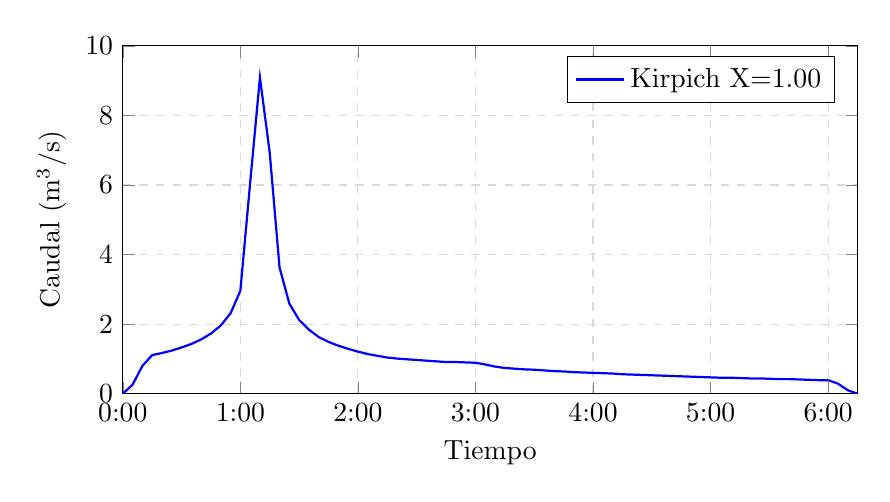
\begin{tikzpicture}
		\begin{axis}[
			width=0.9\textwidth,
			height=6cm,
			xlabel={Tiempo},
			ylabel={Caudal (m$^3$/s)},
			xmin=0,
			xmax=375,
			ymin=0,
			ymax=10,
			grid=major,
			grid style={dashed, gray!30},
			legend pos=north east,
			xtick={0, 60, 120, 180, 240, 300, 360},
			xticklabels={0:00, 1:00, 2:00, 3:00, 4:00, 5:00, 6:00},
			]
		% Kirpich X=1.00
		\addplot [
		blue,
		thick,
		solid,
		] coordinates {
				(0, 0.00) (5, 0.26) (10, 0.80) (15, 1.11) (20, 1.17)
				(25, 1.24) (30, 1.33) (35, 1.43) (40, 1.56) (45, 1.73)
				(50, 1.96) (55, 2.31) (60, 2.96) (65, 6.06) (70, 9.09)
				(75, 6.92) (80, 3.63) (85, 2.59) (90, 2.12) (95, 1.84)
				(100, 1.63) (105, 1.49) (110, 1.38) (115, 1.29) (120, 1.21)
				(125, 1.14) (130, 1.09) (135, 1.04) (140, 1.01) (145, 0.99)
				(150, 0.97) (155, 0.95) (160, 0.93) (165, 0.91) (170, 0.91)
				(175, 0.90) (180, 0.89) (185, 0.84) (190, 0.78) (195, 0.74)
				(200, 0.72) (205, 0.70) (210, 0.69) (215, 0.67) (220, 0.65)
				(225, 0.64) (230, 0.62) (235, 0.61) (240, 0.60) (245, 0.59)
				(250, 0.58) (255, 0.56) (260, 0.55) (265, 0.54) (270, 0.53)
				(275, 0.52) (280, 0.51) (285, 0.50) (290, 0.49) (295, 0.48)
				(300, 0.47) (305, 0.46) (310, 0.46) (315, 0.45) (320, 0.44)
				(325, 0.44) (330, 0.43) (335, 0.42) (340, 0.42) (345, 0.41)
				(350, 0.40) (355, 0.39) (360, 0.39) (365, 0.29) (370, 0.10)
				(375, 0.00)
		};
		\addlegendentry{Kirpich X=1.00}

		\end{axis}
	\end{tikzpicture}
	\caption{Hidrograma - Kirpich + GZ $T_r$=2 años ($Q_p$=9.092 m$^3$/s)}
	\label{fig:hydro_kirpich_gz_Tr2_X100}
\end{figure}
}
\end{minipage}
\caption{Hietograma e Hidrograma - Kirpich + GZ $T_r$=2 años X=1.00}
\end{figure}

\subsection{Kirpich + GZ $T_r$=2 años X=1.25}

% Tabla de parámetros del análisis
\begin{table}[H]
\centering
\small
\begin{tabular}{lr|lr}
\toprule
\multicolumn{2}{c|}{\textbf{Entrada}} & \multicolumn{2}{c}{\textbf{Resultados}} \\
\midrule
Método $T_c$ & Kirpich & Precipitación & 68.6 mm \\
$T_c$ & 12.3 min & Escorrentía & 42.5 mm \\
Tormenta & GZ & $Q_p$ & \textbf{8.201 m$^3$/s} \\
$T_r$ & 2 años & $T_p$ & 70.0 min \\
Factor X & 1.25 & Volumen & 28808 m$^3$ \\
\bottomrule
\end{tabular}
\caption{Ficha técnica: Kirpich + GZ $T_r$=2 años X=1.25}
\end{table}

% Hietograma e Hidrograma
\begin{figure}[H]
\centering
\begin{minipage}{0.48\textwidth}
\centering
\resizebox{\textwidth}{!}{\begin{figure}[H]
	\centering
	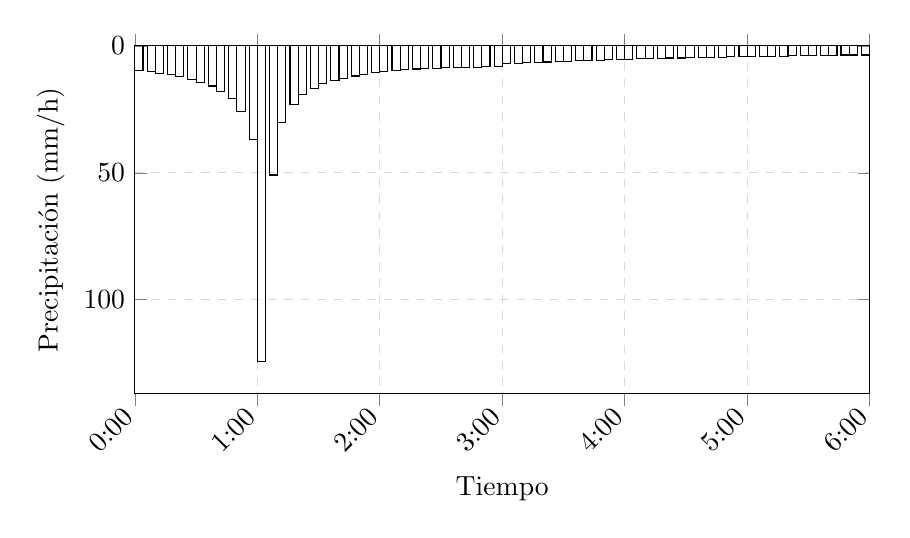
\begin{tikzpicture}
		\begin{axis}[
			width=0.9\textwidth,
			height=6cm,
			xlabel={Tiempo},
			ylabel={Precipitación (mm/h)},
			y dir=reverse,
			ymin=0,
			ymax=137,
			xmin=0,
			xmax=360,
			ybar,
			bar width=4,
			xtick={0, 60, 120, 180, 240, 300, 360},
			xticklabels={0:00, 1:00, 2:00, 3:00, 4:00, 5:00, 6:00},
			xticklabel style={rotate=45, anchor=east},
			grid=major,
			grid style={dashed, gray!30},
			]
			\addplot [
			draw=black,
			fill=none
			]
			coordinates {
				(2, 9.72) (8, 10.20) (12, 10.80) (18, 11.40) (22, 12.24)
				(28, 13.20) (32, 14.40) (38, 15.84) (42, 17.88) (48, 20.88)
				(52, 25.92) (58, 36.96) (62, 124.32) (68, 50.88) (72, 30.12)
				(78, 23.16) (82, 19.32) (88, 16.80) (92, 15.00) (98, 13.68)
				(102, 12.72) (108, 11.88) (112, 11.16) (118, 10.56) (122, 10.08)
				(128, 9.60) (132, 9.36) (138, 9.12) (142, 9.00) (148, 8.76)
				(152, 8.64) (158, 8.40) (162, 8.40) (168, 8.40) (172, 8.16)
				(178, 8.04) (182, 6.96) (188, 6.84) (192, 6.72) (198, 6.48)
				(202, 6.36) (208, 6.24) (212, 6.00) (218, 5.88) (222, 5.76)
				(228, 5.64) (232, 5.52) (238, 5.40) (242, 5.40) (248, 5.16)
				(252, 5.04) (258, 5.04) (262, 4.80) (268, 4.80) (272, 4.68)
				(278, 4.68) (282, 4.56) (288, 4.44) (292, 4.32) (298, 4.32)
				(302, 4.20) (308, 4.20) (312, 4.08) (318, 4.08) (322, 3.96)
				(328, 3.84) (332, 3.84) (338, 3.84) (342, 3.72) (348, 3.60)
				(352, 3.60) (358, 3.60)
			};
		\end{axis}
	\end{tikzpicture}
	\caption{Hietograma - GZ $T_r$=2 años (P=68.6 mm)}
	\label{fig:hyeto_kirpich_gz_Tr2_X125}
\end{figure}
}
\end{minipage}
\hfill
\begin{minipage}{0.48\textwidth}
\centering
\resizebox{\textwidth}{!}{\begin{figure}[H]
	\centering
	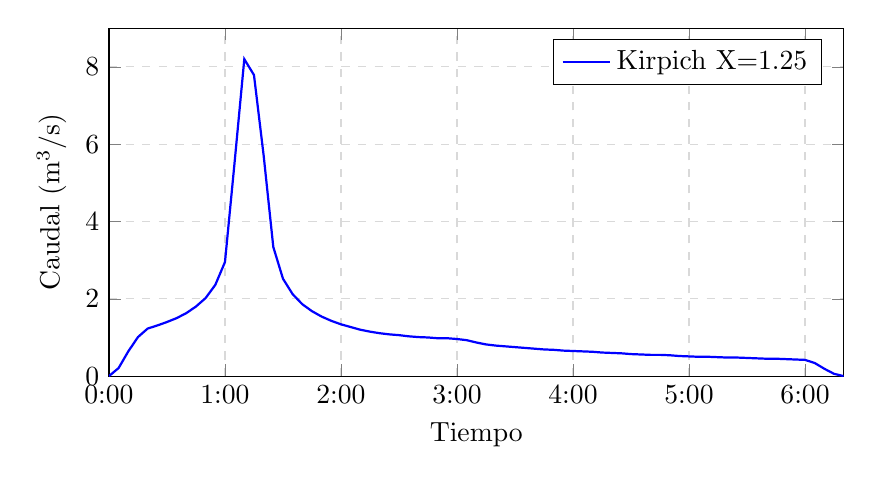
\begin{tikzpicture}
		\begin{axis}[
			width=0.9\textwidth,
			height=6cm,
			xlabel={Tiempo},
			ylabel={Caudal (m$^3$/s)},
			xmin=0,
			xmax=380,
			ymin=0,
			ymax=9,
			grid=major,
			grid style={dashed, gray!30},
			legend pos=north east,
			xtick={0, 60, 120, 180, 240, 300, 360},
			xticklabels={0:00, 1:00, 2:00, 3:00, 4:00, 5:00, 6:00},
			]
		% Kirpich X=1.25
		\addplot [
		blue,
		thick,
		solid,
		] coordinates {
				(0, 0.00) (5, 0.21) (10, 0.64) (15, 1.01) (20, 1.23)
				(25, 1.31) (30, 1.40) (35, 1.50) (40, 1.63) (45, 1.80)
				(50, 2.02) (55, 2.36) (60, 2.95) (65, 5.54) (70, 8.20)
				(75, 7.79) (80, 5.71) (85, 3.34) (90, 2.52) (95, 2.12)
				(100, 1.86) (105, 1.68) (110, 1.54) (115, 1.43) (120, 1.34)
				(125, 1.27) (130, 1.20) (135, 1.15) (140, 1.11) (145, 1.08)
				(150, 1.06) (155, 1.03) (160, 1.01) (165, 1.00) (170, 0.98)
				(175, 0.98) (180, 0.96) (185, 0.93) (190, 0.87) (195, 0.82)
				(200, 0.79) (205, 0.77) (210, 0.75) (215, 0.73) (220, 0.71)
				(225, 0.69) (230, 0.68) (235, 0.66) (240, 0.65) (245, 0.64)
				(250, 0.63) (255, 0.61) (260, 0.60) (265, 0.59) (270, 0.57)
				(275, 0.56) (280, 0.55) (285, 0.55) (290, 0.54) (295, 0.52)
				(300, 0.51) (305, 0.50) (310, 0.50) (315, 0.49) (320, 0.48)
				(325, 0.48) (330, 0.47) (335, 0.46) (340, 0.45) (345, 0.45)
				(350, 0.44) (355, 0.43) (360, 0.42) (365, 0.34) (370, 0.19)
				(375, 0.06) (380, 0.00)
		};
		\addlegendentry{Kirpich X=1.25}

		\end{axis}
	\end{tikzpicture}
	\caption{Hidrograma - Kirpich + GZ $T_r$=2 años ($Q_p$=8.201 m$^3$/s)}
	\label{fig:hydro_kirpich_gz_Tr2_X125}
\end{figure}
}
\end{minipage}
\caption{Hietograma e Hidrograma - Kirpich + GZ $T_r$=2 años X=1.25}
\end{figure}

\subsection{Kirpich + GZ $T_r$=10 años X=1.00}

% Tabla de parámetros del análisis
\begin{table}[H]
\centering
\small
\begin{tabular}{lr|lr}
\toprule
\multicolumn{2}{c|}{\textbf{Entrada}} & \multicolumn{2}{c}{\textbf{Resultados}} \\
\midrule
Método $T_c$ & Kirpich & Precipitación & 105.9 mm \\
$T_c$ & 12.3 min & Escorrentía & 65.7 mm \\
Tormenta & GZ & $Q_p$ & \textbf{14.047 m$^3$/s} \\
$T_r$ & 10 años & $T_p$ & 70.0 min \\
Factor X & 1.00 & Volumen & 41215 m$^3$ \\
\bottomrule
\end{tabular}
\caption{Ficha técnica: Kirpich + GZ $T_r$=10 años X=1.00}
\end{table}

% Hietograma e Hidrograma
\begin{figure}[H]
\centering
\begin{minipage}{0.48\textwidth}
\centering
\resizebox{\textwidth}{!}{\begin{figure}[H]
	\centering
	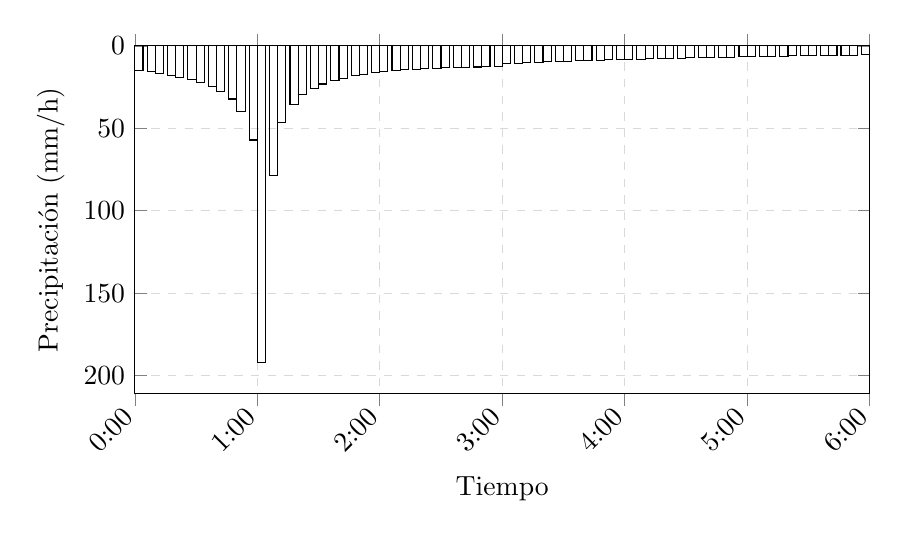
\begin{tikzpicture}
		\begin{axis}[
			width=0.9\textwidth,
			height=6cm,
			xlabel={Tiempo},
			ylabel={Precipitación (mm/h)},
			y dir=reverse,
			ymin=0,
			ymax=211,
			xmin=0,
			xmax=360,
			ybar,
			bar width=4,
			xtick={0, 60, 120, 180, 240, 300, 360},
			xticklabels={0:00, 1:00, 2:00, 3:00, 4:00, 5:00, 6:00},
			xticklabel style={rotate=45, anchor=east},
			grid=major,
			grid style={dashed, gray!30},
			]
			\addplot [
			draw=black,
			fill=none
			]
			coordinates {
				(2, 15.00) (8, 15.84) (12, 16.68) (18, 17.76) (22, 18.96)
				(28, 20.40) (32, 22.20) (38, 24.60) (42, 27.72) (48, 32.28)
				(52, 40.08) (58, 57.12) (62, 192.00) (68, 78.72) (72, 46.56)
				(78, 35.64) (82, 29.76) (88, 25.92) (92, 23.16) (98, 21.24)
				(102, 19.56) (108, 18.24) (112, 17.16) (118, 16.32) (122, 15.48)
				(128, 14.76) (132, 14.52) (138, 14.16) (142, 13.80) (148, 13.56)
				(152, 13.32) (158, 13.08) (162, 12.96) (168, 12.84) (172, 12.60)
				(178, 12.48) (182, 10.92) (188, 10.56) (192, 10.32) (198, 10.08)
				(202, 9.72) (208, 9.60) (212, 9.36) (218, 9.12) (222, 8.88)
				(228, 8.76) (232, 8.52) (238, 8.40) (242, 8.16) (248, 8.04)
				(252, 7.80) (258, 7.68) (262, 7.56) (268, 7.44) (272, 7.20)
				(278, 7.20) (282, 6.96) (288, 6.84) (292, 6.84) (298, 6.60)
				(302, 6.60) (308, 6.36) (312, 6.36) (318, 6.24) (322, 6.12)
				(328, 6.00) (332, 5.88) (338, 5.88) (342, 5.76) (348, 5.64)
				(352, 5.64) (358, 5.52)
			};
		\end{axis}
	\end{tikzpicture}
	\caption{Hietograma - GZ $T_r$=10 años (P=105.9 mm)}
	\label{fig:hyeto_kirpich_gz_Tr10_X100}
\end{figure}
}
\end{minipage}
\hfill
\begin{minipage}{0.48\textwidth}
\centering
\resizebox{\textwidth}{!}{\begin{figure}[H]
	\centering
	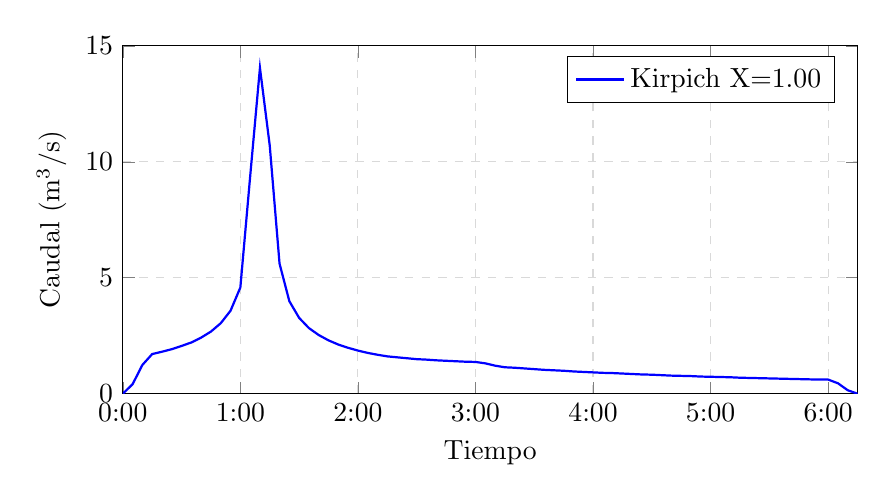
\begin{tikzpicture}
		\begin{axis}[
			width=0.9\textwidth,
			height=6cm,
			xlabel={Tiempo},
			ylabel={Caudal (m$^3$/s)},
			xmin=0,
			xmax=375,
			ymin=0,
			ymax=15,
			grid=major,
			grid style={dashed, gray!30},
			legend pos=north east,
			xtick={0, 60, 120, 180, 240, 300, 360},
			xticklabels={0:00, 1:00, 2:00, 3:00, 4:00, 5:00, 6:00},
			]
		% Kirpich X=1.00
		\addplot [
		blue,
		thick,
		solid,
		] coordinates {
				(0, 0.00) (5, 0.41) (10, 1.24) (15, 1.71) (20, 1.81)
				(25, 1.92) (30, 2.06) (35, 2.21) (40, 2.42) (45, 2.68)
				(50, 3.04) (55, 3.58) (60, 4.58) (65, 9.36) (70, 14.05)
				(75, 10.70) (80, 5.61) (85, 3.99) (90, 3.27) (95, 2.83)
				(100, 2.53) (105, 2.30) (110, 2.12) (115, 1.98) (120, 1.86)
				(125, 1.76) (130, 1.68) (135, 1.61) (140, 1.57) (145, 1.53)
				(150, 1.49) (155, 1.47) (160, 1.44) (165, 1.42) (170, 1.40)
				(175, 1.38) (180, 1.37) (185, 1.31) (190, 1.21) (195, 1.14)
				(200, 1.12) (205, 1.09) (210, 1.06) (215, 1.03) (220, 1.01)
				(225, 0.99) (230, 0.96) (235, 0.94) (240, 0.92) (245, 0.90)
				(250, 0.89) (255, 0.87) (260, 0.85) (265, 0.83) (270, 0.82)
				(275, 0.80) (280, 0.78) (285, 0.77) (290, 0.76) (295, 0.74)
				(300, 0.73) (305, 0.72) (310, 0.71) (315, 0.69) (320, 0.68)
				(325, 0.67) (330, 0.66) (335, 0.65) (340, 0.64) (345, 0.63)
				(350, 0.62) (355, 0.61) (360, 0.61) (365, 0.45) (370, 0.15)
				(375, 0.00)
		};
		\addlegendentry{Kirpich X=1.00}

		\end{axis}
	\end{tikzpicture}
	\caption{Hidrograma - Kirpich + GZ $T_r$=10 años ($Q_p$=14.047 m$^3$/s)}
	\label{fig:hydro_kirpich_gz_Tr10_X100}
\end{figure}
}
\end{minipage}
\caption{Hietograma e Hidrograma - Kirpich + GZ $T_r$=10 años X=1.00}
\end{figure}

\subsection{Kirpich + GZ $T_r$=10 años X=1.25}

% Tabla de parámetros del análisis
\begin{table}[H]
\centering
\small
\begin{tabular}{lr|lr}
\toprule
\multicolumn{2}{c|}{\textbf{Entrada}} & \multicolumn{2}{c}{\textbf{Resultados}} \\
\midrule
Método $T_c$ & Kirpich & Precipitación & 105.9 mm \\
$T_c$ & 12.3 min & Escorrentía & 65.7 mm \\
Tormenta & GZ & $Q_p$ & \textbf{12.672 m$^3$/s} \\
$T_r$ & 10 años & $T_p$ & 70.0 min \\
Factor X & 1.25 & Volumen & 44512 m$^3$ \\
\bottomrule
\end{tabular}
\caption{Ficha técnica: Kirpich + GZ $T_r$=10 años X=1.25}
\end{table}

% Hietograma e Hidrograma
\begin{figure}[H]
\centering
\begin{minipage}{0.48\textwidth}
\centering
\resizebox{\textwidth}{!}{\input{hietograma_kirpich_gz_Tr10_X125.tex}}
\end{minipage}
\hfill
\begin{minipage}{0.48\textwidth}
\centering
\resizebox{\textwidth}{!}{\begin{figure}[H]
	\centering
	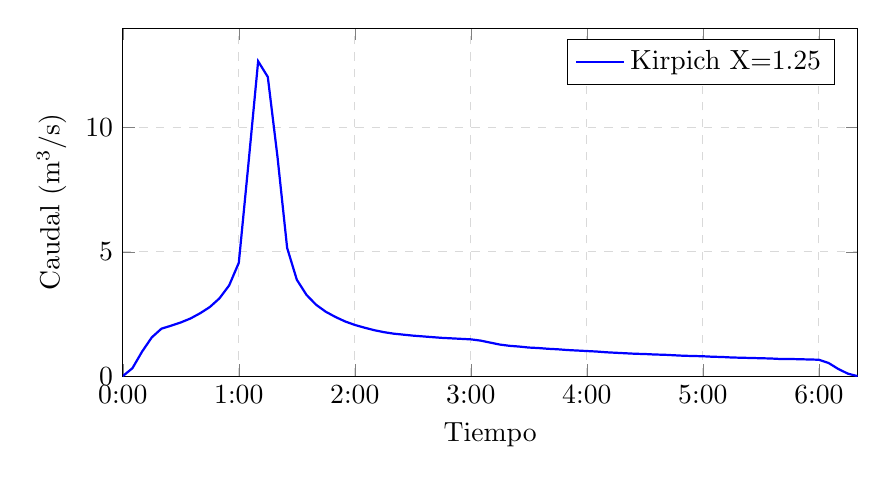
\begin{tikzpicture}
		\begin{axis}[
			width=0.9\textwidth,
			height=6cm,
			xlabel={Tiempo},
			ylabel={Caudal (m$^3$/s)},
			xmin=0,
			xmax=380,
			ymin=0,
			ymax=14,
			grid=major,
			grid style={dashed, gray!30},
			legend pos=north east,
			xtick={0, 60, 120, 180, 240, 300, 360},
			xticklabels={0:00, 1:00, 2:00, 3:00, 4:00, 5:00, 6:00},
			]
		% Kirpich X=1.25
		\addplot [
		blue,
		thick,
		solid,
		] coordinates {
				(0, 0.00) (5, 0.32) (10, 0.99) (15, 1.56) (20, 1.91)
				(25, 2.03) (30, 2.16) (35, 2.32) (40, 2.53) (45, 2.78)
				(50, 3.13) (55, 3.65) (60, 4.56) (65, 8.56) (70, 12.67)
				(75, 12.04) (80, 8.83) (85, 5.16) (90, 3.88) (95, 3.27)
				(100, 2.87) (105, 2.59) (110, 2.38) (115, 2.20) (120, 2.06)
				(125, 1.95) (130, 1.85) (135, 1.77) (140, 1.71) (145, 1.67)
				(150, 1.63) (155, 1.60) (160, 1.57) (165, 1.54) (170, 1.52)
				(175, 1.50) (180, 1.48) (185, 1.43) (190, 1.35) (195, 1.27)
				(200, 1.22) (205, 1.19) (210, 1.15) (215, 1.13) (220, 1.10)
				(225, 1.08) (230, 1.05) (235, 1.03) (240, 1.01) (245, 0.99)
				(250, 0.96) (255, 0.94) (260, 0.92) (265, 0.90) (270, 0.89)
				(275, 0.87) (280, 0.86) (285, 0.84) (290, 0.82) (295, 0.81)
				(300, 0.80) (305, 0.78) (310, 0.77) (315, 0.75) (320, 0.74)
				(325, 0.73) (330, 0.72) (335, 0.71) (340, 0.69) (345, 0.69)
				(350, 0.68) (355, 0.67) (360, 0.66) (365, 0.53) (370, 0.29)
				(375, 0.10) (380, 0.00)
		};
		\addlegendentry{Kirpich X=1.25}

		\end{axis}
	\end{tikzpicture}
	\caption{Hidrograma - Kirpich + GZ $T_r$=10 años ($Q_p$=12.672 m$^3$/s)}
	\label{fig:hydro_kirpich_gz_Tr10_X125}
\end{figure}
}
\end{minipage}
\caption{Hietograma e Hidrograma - Kirpich + GZ $T_r$=10 años X=1.25}
\end{figure}

\subsection{Kirpich + GZ $T_r$=25 años X=1.00}

% Tabla de parámetros del análisis
\begin{table}[H]
\centering
\small
\begin{tabular}{lr|lr}
\toprule
\multicolumn{2}{c|}{\textbf{Entrada}} & \multicolumn{2}{c}{\textbf{Resultados}} \\
\midrule
Método $T_c$ & Kirpich & Precipitación & 124.7 mm \\
$T_c$ & 12.3 min & Escorrentía & 77.3 mm \\
Tormenta & GZ & $Q_p$ & \textbf{16.541 m$^3$/s} \\
$T_r$ & 25 años & $T_p$ & 70.0 min \\
Factor X & 1.00 & Volumen & 48530 m$^3$ \\
\bottomrule
\end{tabular}
\caption{Ficha técnica: Kirpich + GZ $T_r$=25 años X=1.00}
\end{table}

% Hietograma e Hidrograma
\begin{figure}[H]
\centering
\begin{minipage}{0.48\textwidth}
\centering
\resizebox{\textwidth}{!}{\input{hietograma_kirpich_gz_Tr25_X100.tex}}
\end{minipage}
\hfill
\begin{minipage}{0.48\textwidth}
\centering
\resizebox{\textwidth}{!}{\begin{figure}[H]
	\centering
	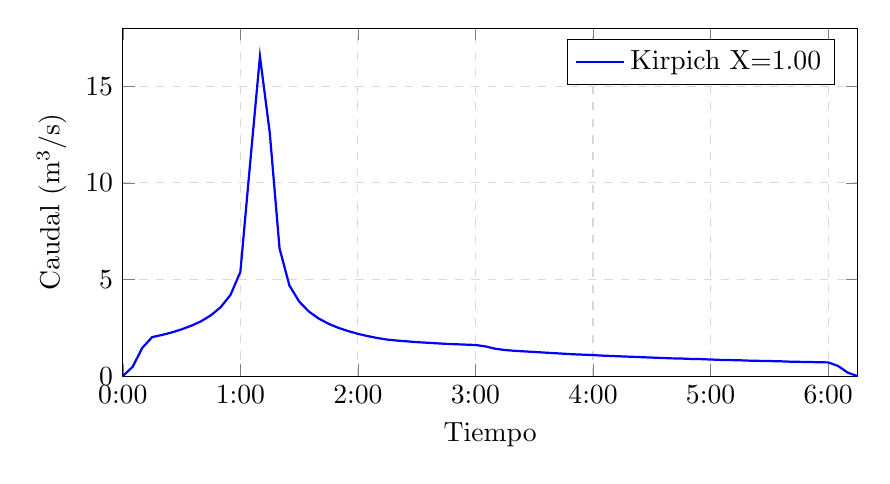
\begin{tikzpicture}
		\begin{axis}[
			width=0.9\textwidth,
			height=6cm,
			xlabel={Tiempo},
			ylabel={Caudal (m$^3$/s)},
			xmin=0,
			xmax=375,
			ymin=0,
			ymax=18,
			grid=major,
			grid style={dashed, gray!30},
			legend pos=north east,
			xtick={0, 60, 120, 180, 240, 300, 360},
			xticklabels={0:00, 1:00, 2:00, 3:00, 4:00, 5:00, 6:00},
			]
		% Kirpich X=1.00
		\addplot [
		blue,
		thick,
		solid,
		] coordinates {
				(0, 0.00) (5, 0.48) (10, 1.47) (15, 2.02) (20, 2.13)
				(25, 2.26) (30, 2.42) (35, 2.61) (40, 2.84) (45, 3.15)
				(50, 3.57) (55, 4.21) (60, 5.39) (65, 11.02) (70, 16.54)
				(75, 12.60) (80, 6.61) (85, 4.70) (90, 3.86) (95, 3.34)
				(100, 2.98) (105, 2.71) (110, 2.50) (115, 2.33) (120, 2.19)
				(125, 2.07) (130, 1.97) (135, 1.89) (140, 1.84) (145, 1.80)
				(150, 1.76) (155, 1.73) (160, 1.70) (165, 1.67) (170, 1.65)
				(175, 1.63) (180, 1.61) (185, 1.54) (190, 1.42) (195, 1.35)
				(200, 1.31) (205, 1.28) (210, 1.25) (215, 1.22) (220, 1.19)
				(225, 1.16) (230, 1.13) (235, 1.11) (240, 1.09) (245, 1.06)
				(250, 1.04) (255, 1.02) (260, 1.00) (265, 0.98) (270, 0.96)
				(275, 0.94) (280, 0.92) (285, 0.91) (290, 0.89) (295, 0.88)
				(300, 0.86) (305, 0.84) (310, 0.83) (315, 0.82) (320, 0.80)
				(325, 0.79) (330, 0.78) (335, 0.77) (340, 0.75) (345, 0.74)
				(350, 0.73) (355, 0.72) (360, 0.71) (365, 0.53) (370, 0.18)
				(375, 0.00)
		};
		\addlegendentry{Kirpich X=1.00}

		\end{axis}
	\end{tikzpicture}
	\caption{Hidrograma - Kirpich + GZ $T_r$=25 años ($Q_p$=16.541 m$^3$/s)}
	\label{fig:hydro_kirpich_gz_Tr25_X100}
\end{figure}
}
\end{minipage}
\caption{Hietograma e Hidrograma - Kirpich + GZ $T_r$=25 años X=1.00}
\end{figure}

\subsection{Kirpich + GZ $T_r$=25 años X=1.25}

% Tabla de parámetros del análisis
\begin{table}[H]
\centering
\small
\begin{tabular}{lr|lr}
\toprule
\multicolumn{2}{c|}{\textbf{Entrada}} & \multicolumn{2}{c}{\textbf{Resultados}} \\
\midrule
Método $T_c$ & Kirpich & Precipitación & 124.7 mm \\
$T_c$ & 12.3 min & Escorrentía & 77.3 mm \\
Tormenta & GZ & $Q_p$ & \textbf{14.920 m$^3$/s} \\
$T_r$ & 25 años & $T_p$ & 70.0 min \\
Factor X & 1.25 & Volumen & 52413 m$^3$ \\
\bottomrule
\end{tabular}
\caption{Ficha técnica: Kirpich + GZ $T_r$=25 años X=1.25}
\end{table}

% Hietograma e Hidrograma
\begin{figure}[H]
\centering
\begin{minipage}{0.48\textwidth}
\centering
\resizebox{\textwidth}{!}{\begin{figure}[H]
	\centering
	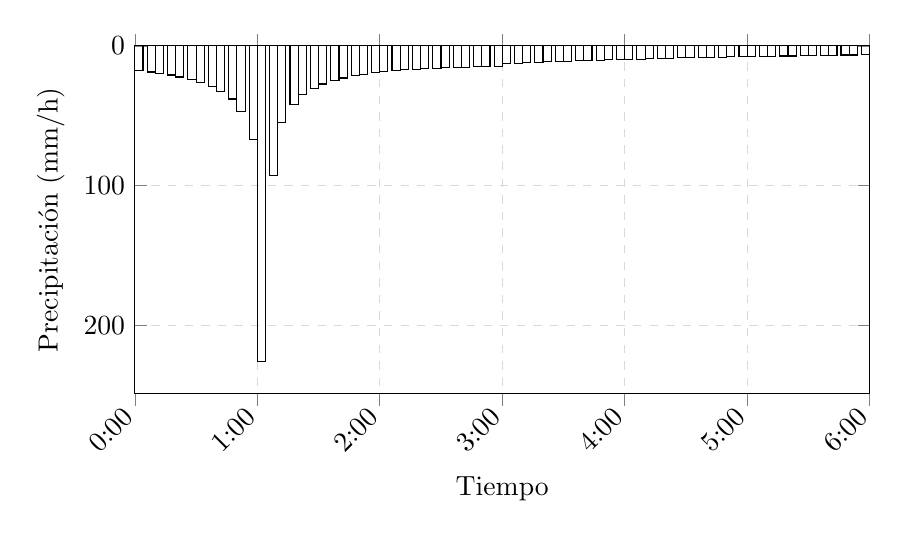
\begin{tikzpicture}
		\begin{axis}[
			width=0.9\textwidth,
			height=6cm,
			xlabel={Tiempo},
			ylabel={Precipitación (mm/h)},
			y dir=reverse,
			ymin=0,
			ymax=249,
			xmin=0,
			xmax=360,
			ybar,
			bar width=4,
			xtick={0, 60, 120, 180, 240, 300, 360},
			xticklabels={0:00, 1:00, 2:00, 3:00, 4:00, 5:00, 6:00},
			xticklabel style={rotate=45, anchor=east},
			grid=major,
			grid style={dashed, gray!30},
			]
			\addplot [
			draw=black,
			fill=none
			]
			coordinates {
				(2, 17.76) (8, 18.72) (12, 19.68) (18, 20.88) (22, 22.32)
				(28, 24.00) (32, 26.16) (38, 28.80) (42, 32.64) (48, 38.04)
				(52, 47.16) (58, 67.20) (62, 226.08) (68, 92.76) (72, 54.84)
				(78, 42.00) (82, 35.04) (88, 30.60) (92, 27.36) (98, 24.96)
				(102, 23.04) (108, 21.48) (112, 20.28) (118, 19.08) (122, 18.24)
				(128, 17.40) (132, 16.92) (138, 16.68) (142, 16.32) (148, 15.96)
				(152, 15.72) (158, 15.48) (162, 15.24) (168, 15.12) (172, 14.88)
				(178, 14.64) (182, 12.72) (188, 12.48) (192, 12.12) (198, 11.88)
				(202, 11.52) (208, 11.28) (212, 11.04) (218, 10.68) (222, 10.56)
				(228, 10.20) (232, 10.08) (238, 9.84) (242, 9.60) (248, 9.48)
				(252, 9.24) (258, 9.00) (262, 9.00) (268, 8.64) (272, 8.52)
				(278, 8.40) (282, 8.28) (288, 8.16) (292, 7.92) (298, 7.80)
				(302, 7.68) (308, 7.56) (312, 7.44) (318, 7.32) (322, 7.32)
				(328, 7.08) (332, 6.96) (338, 6.84) (342, 6.84) (348, 6.60)
				(352, 6.60) (358, 6.48)
			};
		\end{axis}
	\end{tikzpicture}
	\caption{Hietograma - GZ $T_r$=25 años (P=124.7 mm)}
	\label{fig:hyeto_kirpich_gz_Tr25_X125}
\end{figure}
}
\end{minipage}
\hfill
\begin{minipage}{0.48\textwidth}
\centering
\resizebox{\textwidth}{!}{\begin{figure}[H]
	\centering
	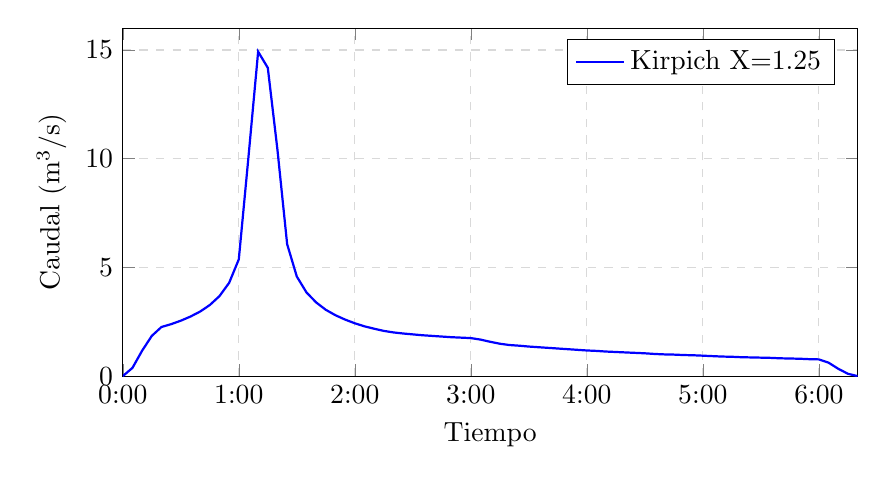
\begin{tikzpicture}
		\begin{axis}[
			width=0.9\textwidth,
			height=6cm,
			xlabel={Tiempo},
			ylabel={Caudal (m$^3$/s)},
			xmin=0,
			xmax=380,
			ymin=0,
			ymax=16,
			grid=major,
			grid style={dashed, gray!30},
			legend pos=north east,
			xtick={0, 60, 120, 180, 240, 300, 360},
			xticklabels={0:00, 1:00, 2:00, 3:00, 4:00, 5:00, 6:00},
			]
		% Kirpich X=1.25
		\addplot [
		blue,
		thick,
		solid,
		] coordinates {
				(0, 0.00) (5, 0.38) (10, 1.17) (15, 1.85) (20, 2.26)
				(25, 2.39) (30, 2.55) (35, 2.74) (40, 2.97) (45, 3.27)
				(50, 3.68) (55, 4.29) (60, 5.37) (65, 10.08) (70, 14.92)
				(75, 14.18) (80, 10.40) (85, 6.07) (90, 4.58) (95, 3.85)
				(100, 3.39) (105, 3.05) (110, 2.80) (115, 2.60) (120, 2.43)
				(125, 2.29) (130, 2.18) (135, 2.08) (140, 2.01) (145, 1.96)
				(150, 1.92) (155, 1.88) (160, 1.85) (165, 1.82) (170, 1.79)
				(175, 1.77) (180, 1.75) (185, 1.68) (190, 1.58) (195, 1.49)
				(200, 1.43) (205, 1.40) (210, 1.36) (215, 1.33) (220, 1.30)
				(225, 1.27) (230, 1.24) (235, 1.21) (240, 1.18) (245, 1.16)
				(250, 1.13) (255, 1.11) (260, 1.09) (265, 1.07) (270, 1.05)
				(275, 1.02) (280, 1.00) (285, 0.99) (290, 0.97) (295, 0.96)
				(300, 0.94) (305, 0.92) (310, 0.90) (315, 0.89) (320, 0.87)
				(325, 0.86) (330, 0.85) (335, 0.84) (340, 0.82) (345, 0.81)
				(350, 0.80) (355, 0.78) (360, 0.77) (365, 0.62) (370, 0.34)
				(375, 0.11) (380, 0.00)
		};
		\addlegendentry{Kirpich X=1.25}

		\end{axis}
	\end{tikzpicture}
	\caption{Hidrograma - Kirpich + GZ $T_r$=25 años ($Q_p$=14.920 m$^3$/s)}
	\label{fig:hydro_kirpich_gz_Tr25_X125}
\end{figure}
}
\end{minipage}
\caption{Hietograma e Hidrograma - Kirpich + GZ $T_r$=25 años X=1.25}
\end{figure}

\subsection{Desbordes + GZ $T_r$=2 años X=1.00}

% Tabla de parámetros del análisis
\begin{table}[H]
\centering
\small
\begin{tabular}{lr|lr}
\toprule
\multicolumn{2}{c|}{\textbf{Entrada}} & \multicolumn{2}{c}{\textbf{Resultados}} \\
\midrule
Método $T_c$ & Desbordes & Precipitación & 68.6 mm \\
$T_c$ & 22.6 min & Escorrentía & 42.5 mm \\
Tormenta & GZ & $Q_p$ & \textbf{6.748 m$^3$/s} \\
$T_r$ & 2 años & $T_p$ & 80.0 min \\
Factor X & 1.00 & Volumen & 28191 m$^3$ \\
\bottomrule
\end{tabular}
\caption{Ficha técnica: Desbordes + GZ $T_r$=2 años X=1.00}
\end{table}

% Hietograma e Hidrograma
\begin{figure}[H]
\centering
\begin{minipage}{0.48\textwidth}
\centering
\resizebox{\textwidth}{!}{\input{hietograma_desbordes_gz_Tr2_X100.tex}}
\end{minipage}
\hfill
\begin{minipage}{0.48\textwidth}
\centering
\resizebox{\textwidth}{!}{\begin{figure}[H]
	\centering
	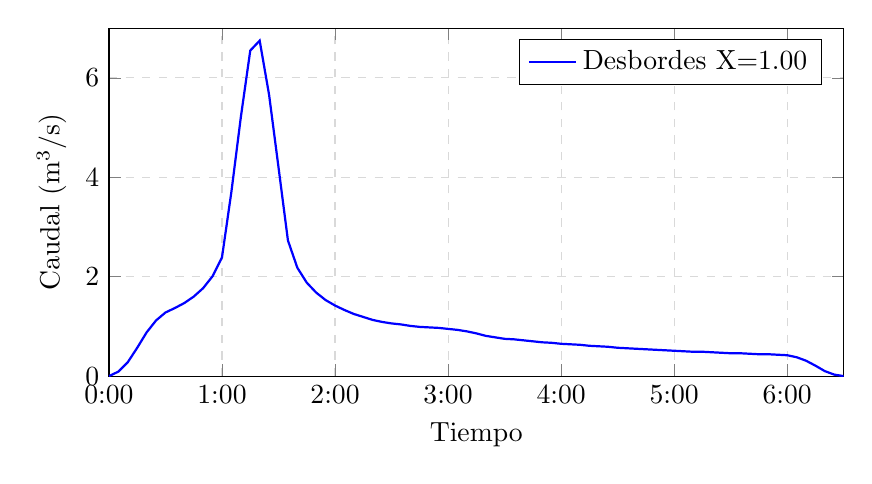
\begin{tikzpicture}
		\begin{axis}[
			width=0.9\textwidth,
			height=6cm,
			xlabel={Tiempo},
			ylabel={Caudal (m$^3$/s)},
			xmin=0,
			xmax=390,
			ymin=0,
			ymax=7,
			grid=major,
			grid style={dashed, gray!30},
			legend pos=north east,
			xtick={0, 60, 120, 180, 240, 300, 360},
			xticklabels={0:00, 1:00, 2:00, 3:00, 4:00, 5:00, 6:00},
			]
		% Desbordes X=1.00
		\addplot [
		blue,
		thick,
		solid,
		] coordinates {
				(0, 0.00) (5, 0.09) (10, 0.28) (15, 0.57) (20, 0.88)
				(25, 1.12) (30, 1.28) (35, 1.37) (40, 1.47) (45, 1.60)
				(50, 1.77) (55, 2.01) (60, 2.39) (65, 3.71) (70, 5.21)
				(75, 6.55) (80, 6.75) (85, 5.66) (90, 4.20) (95, 2.73)
				(100, 2.18) (105, 1.88) (110, 1.68) (115, 1.53) (120, 1.42)
				(125, 1.33) (130, 1.25) (135, 1.19) (140, 1.13) (145, 1.09)
				(150, 1.06) (155, 1.04) (160, 1.01) (165, 0.99) (170, 0.98)
				(175, 0.97) (180, 0.95) (185, 0.93) (190, 0.90) (195, 0.86)
				(200, 0.81) (205, 0.78) (210, 0.75) (215, 0.74) (220, 0.72)
				(225, 0.70) (230, 0.68) (235, 0.67) (240, 0.65) (245, 0.64)
				(250, 0.63) (255, 0.61) (260, 0.60) (265, 0.59) (270, 0.57)
				(275, 0.56) (280, 0.55) (285, 0.54) (290, 0.53) (295, 0.52)
				(300, 0.51) (305, 0.50) (310, 0.49) (315, 0.49) (320, 0.48)
				(325, 0.47) (330, 0.46) (335, 0.46) (340, 0.45) (345, 0.44)
				(350, 0.44) (355, 0.43) (360, 0.42) (365, 0.38) (370, 0.31)
				(375, 0.21) (380, 0.10) (385, 0.03) (390, 0.00)
		};
		\addlegendentry{Desbordes X=1.00}

		\end{axis}
	\end{tikzpicture}
	\caption{Hidrograma - Desbordes + GZ $T_r$=2 años ($Q_p$=6.748 m$^3$/s)}
	\label{fig:hydro_desbordes_gz_Tr2_X100}
\end{figure}
}
\end{minipage}
\caption{Hietograma e Hidrograma - Desbordes + GZ $T_r$=2 años X=1.00}
\end{figure}

\subsection{Desbordes + GZ $T_r$=2 años X=1.25}

% Tabla de parámetros del análisis
\begin{table}[H]
\centering
\small
\begin{tabular}{lr|lr}
\toprule
\multicolumn{2}{c|}{\textbf{Entrada}} & \multicolumn{2}{c}{\textbf{Resultados}} \\
\midrule
Método $T_c$ & Desbordes & Precipitación & 68.6 mm \\
$T_c$ & 22.6 min & Escorrentía & 42.5 mm \\
Tormenta & GZ & $Q_p$ & \textbf{6.503 m$^3$/s} \\
$T_r$ & 2 años & $T_p$ & 80.0 min \\
Factor X & 1.25 & Volumen & 28778 m$^3$ \\
\bottomrule
\end{tabular}
\caption{Ficha técnica: Desbordes + GZ $T_r$=2 años X=1.25}
\end{table}

% Hietograma e Hidrograma
\begin{figure}[H]
\centering
\begin{minipage}{0.48\textwidth}
\centering
\resizebox{\textwidth}{!}{\input{hietograma_desbordes_gz_Tr2_X125.tex}}
\end{minipage}
\hfill
\begin{minipage}{0.48\textwidth}
\centering
\resizebox{\textwidth}{!}{\begin{figure}[H]
	\centering
	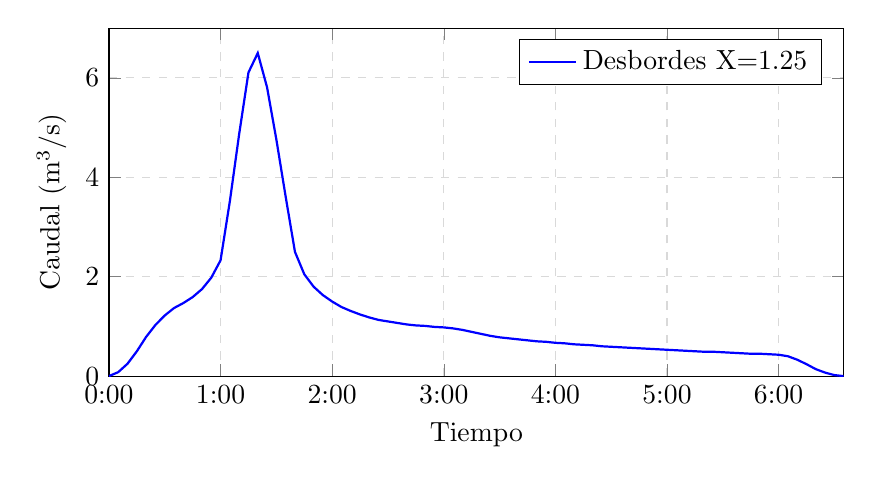
\begin{tikzpicture}
		\begin{axis}[
			width=0.9\textwidth,
			height=6cm,
			xlabel={Tiempo},
			ylabel={Caudal (m$^3$/s)},
			xmin=0,
			xmax=395,
			ymin=0,
			ymax=7,
			grid=major,
			grid style={dashed, gray!30},
			legend pos=north east,
			xtick={0, 60, 120, 180, 240, 300, 360},
			xticklabels={0:00, 1:00, 2:00, 3:00, 4:00, 5:00, 6:00},
			]
		% Desbordes X=1.25
		\addplot [
		blue,
		thick,
		solid,
		] coordinates {
				(0, 0.00) (5, 0.08) (10, 0.25) (15, 0.50) (20, 0.79)
				(25, 1.03) (30, 1.22) (35, 1.37) (40, 1.47) (45, 1.59)
				(50, 1.75) (55, 1.98) (60, 2.33) (65, 3.52) (70, 4.87)
				(75, 6.11) (80, 6.50) (85, 5.81) (90, 4.76) (95, 3.61)
				(100, 2.50) (105, 2.05) (110, 1.80) (115, 1.63) (120, 1.50)
				(125, 1.39) (130, 1.31) (135, 1.24) (140, 1.18) (145, 1.13)
				(150, 1.10) (155, 1.07) (160, 1.04) (165, 1.02) (170, 1.01)
				(175, 0.99) (180, 0.98) (185, 0.96) (190, 0.93) (195, 0.89)
				(200, 0.85) (205, 0.81) (210, 0.78) (215, 0.76) (220, 0.74)
				(225, 0.72) (230, 0.70) (235, 0.69) (240, 0.67) (245, 0.66)
				(250, 0.64) (255, 0.63) (260, 0.62) (265, 0.60) (270, 0.59)
				(275, 0.58) (280, 0.57) (285, 0.56) (290, 0.55) (295, 0.54)
				(300, 0.53) (305, 0.52) (310, 0.51) (315, 0.50) (320, 0.49)
				(325, 0.49) (330, 0.48) (335, 0.47) (340, 0.46) (345, 0.45)
				(350, 0.45) (355, 0.44) (360, 0.43) (365, 0.40) (370, 0.33)
				(375, 0.24) (380, 0.14) (385, 0.07) (390, 0.02) (395, 0.00)
		};
		\addlegendentry{Desbordes X=1.25}

		\end{axis}
	\end{tikzpicture}
	\caption{Hidrograma - Desbordes + GZ $T_r$=2 años ($Q_p$=6.503 m$^3$/s)}
	\label{fig:hydro_desbordes_gz_Tr2_X125}
\end{figure}
}
\end{minipage}
\caption{Hietograma e Hidrograma - Desbordes + GZ $T_r$=2 años X=1.25}
\end{figure}

\subsection{Desbordes + GZ $T_r$=10 años X=1.00}

% Tabla de parámetros del análisis
\begin{table}[H]
\centering
\small
\begin{tabular}{lr|lr}
\toprule
\multicolumn{2}{c|}{\textbf{Entrada}} & \multicolumn{2}{c}{\textbf{Resultados}} \\
\midrule
Método $T_c$ & Desbordes & Precipitación & 105.9 mm \\
$T_c$ & 22.6 min & Escorrentía & 65.7 mm \\
Tormenta & GZ & $Q_p$ & \textbf{10.426 m$^3$/s} \\
$T_r$ & 10 años & $T_p$ & 80.0 min \\
Factor X & 1.00 & Volumen & 43559 m$^3$ \\
\bottomrule
\end{tabular}
\caption{Ficha técnica: Desbordes + GZ $T_r$=10 años X=1.00}
\end{table}

% Hietograma e Hidrograma
\begin{figure}[H]
\centering
\begin{minipage}{0.48\textwidth}
\centering
\resizebox{\textwidth}{!}{\input{hietograma_desbordes_gz_Tr10_X100.tex}}
\end{minipage}
\hfill
\begin{minipage}{0.48\textwidth}
\centering
\resizebox{\textwidth}{!}{\begin{figure}[H]
	\centering
	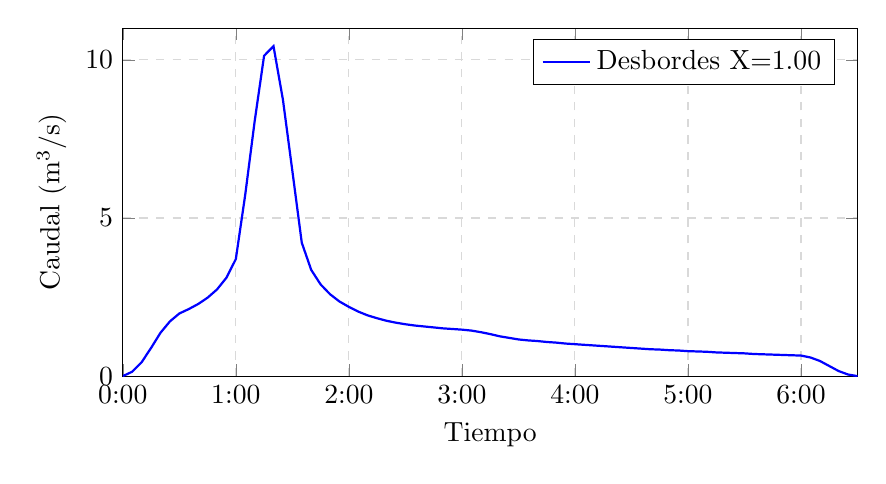
\begin{tikzpicture}
		\begin{axis}[
			width=0.9\textwidth,
			height=6cm,
			xlabel={Tiempo},
			ylabel={Caudal (m$^3$/s)},
			xmin=0,
			xmax=390,
			ymin=0,
			ymax=11,
			grid=major,
			grid style={dashed, gray!30},
			legend pos=north east,
			xtick={0, 60, 120, 180, 240, 300, 360},
			xticklabels={0:00, 1:00, 2:00, 3:00, 4:00, 5:00, 6:00},
			]
		% Desbordes X=1.00
		\addplot [
		blue,
		thick,
		solid,
		] coordinates {
				(0, 0.00) (5, 0.14) (10, 0.44) (15, 0.89) (20, 1.37)
				(25, 1.73) (30, 1.98) (35, 2.12) (40, 2.28) (45, 2.48)
				(50, 2.74) (55, 3.11) (60, 3.70) (65, 5.74) (70, 8.06)
				(75, 10.13) (80, 10.43) (85, 8.74) (90, 6.49) (95, 4.22)
				(100, 3.36) (105, 2.90) (110, 2.59) (115, 2.36) (120, 2.19)
				(125, 2.04) (130, 1.92) (135, 1.83) (140, 1.75) (145, 1.69)
				(150, 1.64) (155, 1.60) (160, 1.57) (165, 1.54) (170, 1.51)
				(175, 1.49) (180, 1.47) (185, 1.44) (190, 1.39) (195, 1.33)
				(200, 1.26) (205, 1.21) (210, 1.16) (215, 1.13) (220, 1.11)
				(225, 1.08) (230, 1.06) (235, 1.03) (240, 1.01) (245, 0.99)
				(250, 0.97) (255, 0.95) (260, 0.93) (265, 0.91) (270, 0.89)
				(275, 0.87) (280, 0.85) (285, 0.84) (290, 0.82) (295, 0.81)
				(300, 0.79) (305, 0.78) (310, 0.77) (315, 0.75) (320, 0.74)
				(325, 0.73) (330, 0.72) (335, 0.70) (340, 0.69) (345, 0.68)
				(350, 0.67) (355, 0.66) (360, 0.65) (365, 0.59) (370, 0.48)
				(375, 0.32) (380, 0.16) (385, 0.05) (390, 0.00)
		};
		\addlegendentry{Desbordes X=1.00}

		\end{axis}
	\end{tikzpicture}
	\caption{Hidrograma - Desbordes + GZ $T_r$=10 años ($Q_p$=10.426 m$^3$/s)}
	\label{fig:hydro_desbordes_gz_Tr10_X100}
\end{figure}
}
\end{minipage}
\caption{Hietograma e Hidrograma - Desbordes + GZ $T_r$=10 años X=1.00}
\end{figure}

\subsection{Desbordes + GZ $T_r$=10 años X=1.25}

% Tabla de parámetros del análisis
\begin{table}[H]
\centering
\small
\begin{tabular}{lr|lr}
\toprule
\multicolumn{2}{c|}{\textbf{Entrada}} & \multicolumn{2}{c}{\textbf{Resultados}} \\
\midrule
Método $T_c$ & Desbordes & Precipitación & 105.9 mm \\
$T_c$ & 22.6 min & Escorrentía & 65.7 mm \\
Tormenta & GZ & $Q_p$ & \textbf{10.048 m$^3$/s} \\
$T_r$ & 10 años & $T_p$ & 80.0 min \\
Factor X & 1.25 & Volumen & 44466 m$^3$ \\
\bottomrule
\end{tabular}
\caption{Ficha técnica: Desbordes + GZ $T_r$=10 años X=1.25}
\end{table}

% Hietograma e Hidrograma
\begin{figure}[H]
\centering
\begin{minipage}{0.48\textwidth}
\centering
\resizebox{\textwidth}{!}{\input{hietograma_desbordes_gz_Tr10_X125.tex}}
\end{minipage}
\hfill
\begin{minipage}{0.48\textwidth}
\centering
\resizebox{\textwidth}{!}{\begin{figure}[H]
	\centering
	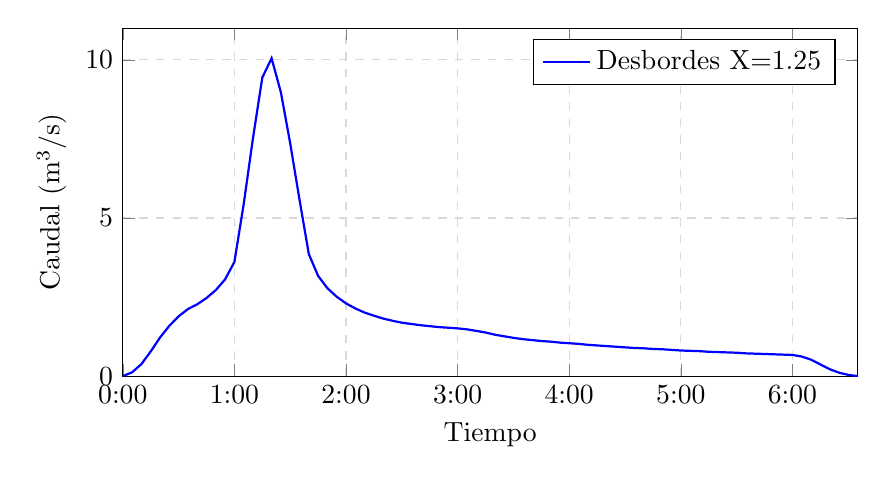
\begin{tikzpicture}
		\begin{axis}[
			width=0.9\textwidth,
			height=6cm,
			xlabel={Tiempo},
			ylabel={Caudal (m$^3$/s)},
			xmin=0,
			xmax=395,
			ymin=0,
			ymax=11,
			grid=major,
			grid style={dashed, gray!30},
			legend pos=north east,
			xtick={0, 60, 120, 180, 240, 300, 360},
			xticklabels={0:00, 1:00, 2:00, 3:00, 4:00, 5:00, 6:00},
			]
		% Desbordes X=1.25
		\addplot [
		blue,
		thick,
		solid,
		] coordinates {
				(0, 0.00) (5, 0.12) (10, 0.38) (15, 0.78) (20, 1.22)
				(25, 1.59) (30, 1.89) (35, 2.12) (40, 2.27) (45, 2.47)
				(50, 2.72) (55, 3.06) (60, 3.61) (65, 5.44) (70, 7.53)
				(75, 9.44) (80, 10.05) (85, 8.97) (90, 7.36) (95, 5.58)
				(100, 3.86) (105, 3.17) (110, 2.78) (115, 2.51) (120, 2.30)
				(125, 2.14) (130, 2.01) (135, 1.91) (140, 1.82) (145, 1.75)
				(150, 1.69) (155, 1.65) (160, 1.61) (165, 1.58) (170, 1.55)
				(175, 1.53) (180, 1.51) (185, 1.48) (190, 1.43) (195, 1.38)
				(200, 1.31) (205, 1.26) (210, 1.21) (215, 1.17) (220, 1.14)
				(225, 1.11) (230, 1.09) (235, 1.06) (240, 1.04) (245, 1.02)
				(250, 0.99) (255, 0.97) (260, 0.95) (265, 0.93) (270, 0.91)
				(275, 0.89) (280, 0.88) (285, 0.86) (290, 0.85) (295, 0.83)
				(300, 0.81) (305, 0.80) (310, 0.79) (315, 0.77) (320, 0.76)
				(325, 0.75) (330, 0.74) (335, 0.72) (340, 0.71) (345, 0.70)
				(350, 0.69) (355, 0.68) (360, 0.67) (365, 0.62) (370, 0.52)
				(375, 0.37) (380, 0.22) (385, 0.11) (390, 0.04) (395, 0.00)
		};
		\addlegendentry{Desbordes X=1.25}

		\end{axis}
	\end{tikzpicture}
	\caption{Hidrograma - Desbordes + GZ $T_r$=10 años ($Q_p$=10.048 m$^3$/s)}
	\label{fig:hydro_desbordes_gz_Tr10_X125}
\end{figure}
}
\end{minipage}
\caption{Hietograma e Hidrograma - Desbordes + GZ $T_r$=10 años X=1.25}
\end{figure}

\subsection{Desbordes + GZ $T_r$=25 años X=1.00}

% Tabla de parámetros del análisis
\begin{table}[H]
\centering
\small
\begin{tabular}{lr|lr}
\toprule
\multicolumn{2}{c|}{\textbf{Entrada}} & \multicolumn{2}{c}{\textbf{Resultados}} \\
\midrule
Método $T_c$ & Desbordes & Precipitación & 124.7 mm \\
$T_c$ & 22.6 min & Escorrentía & 77.3 mm \\
Tormenta & GZ & $Q_p$ & \textbf{12.278 m$^3$/s} \\
$T_r$ & 25 años & $T_p$ & 80.0 min \\
Factor X & 1.00 & Volumen & 51290 m$^3$ \\
\bottomrule
\end{tabular}
\caption{Ficha técnica: Desbordes + GZ $T_r$=25 años X=1.00}
\end{table}

% Hietograma e Hidrograma
\begin{figure}[H]
\centering
\begin{minipage}{0.48\textwidth}
\centering
\resizebox{\textwidth}{!}{\input{hietograma_desbordes_gz_Tr25_X100.tex}}
\end{minipage}
\hfill
\begin{minipage}{0.48\textwidth}
\centering
\resizebox{\textwidth}{!}{\begin{figure}[H]
	\centering
	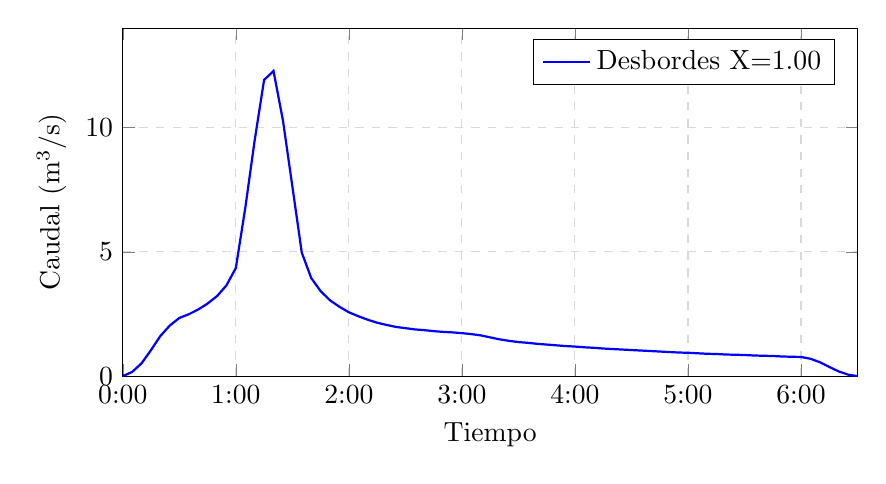
\begin{tikzpicture}
		\begin{axis}[
			width=0.9\textwidth,
			height=6cm,
			xlabel={Tiempo},
			ylabel={Caudal (m$^3$/s)},
			xmin=0,
			xmax=390,
			ymin=0,
			ymax=14,
			grid=major,
			grid style={dashed, gray!30},
			legend pos=north east,
			xtick={0, 60, 120, 180, 240, 300, 360},
			xticklabels={0:00, 1:00, 2:00, 3:00, 4:00, 5:00, 6:00},
			]
		% Desbordes X=1.00
		\addplot [
		blue,
		thick,
		solid,
		] coordinates {
				(0, 0.00) (5, 0.17) (10, 0.52) (15, 1.05) (20, 1.62)
				(25, 2.04) (30, 2.34) (35, 2.49) (40, 2.68) (45, 2.92)
				(50, 3.22) (55, 3.65) (60, 4.35) (65, 6.76) (70, 9.49)
				(75, 11.92) (80, 12.28) (85, 10.29) (90, 7.64) (95, 4.97)
				(100, 3.95) (105, 3.42) (110, 3.05) (115, 2.79) (120, 2.57)
				(125, 2.41) (130, 2.27) (135, 2.15) (140, 2.06) (145, 1.98)
				(150, 1.93) (155, 1.88) (160, 1.85) (165, 1.81) (170, 1.78)
				(175, 1.76) (180, 1.73) (185, 1.69) (190, 1.64) (195, 1.56)
				(200, 1.48) (205, 1.42) (210, 1.37) (215, 1.34) (220, 1.30)
				(225, 1.27) (230, 1.24) (235, 1.21) (240, 1.19) (245, 1.16)
				(250, 1.14) (255, 1.11) (260, 1.09) (265, 1.07) (270, 1.05)
				(275, 1.03) (280, 1.01) (285, 0.99) (290, 0.97) (295, 0.95)
				(300, 0.94) (305, 0.92) (310, 0.90) (315, 0.89) (320, 0.87)
				(325, 0.86) (330, 0.85) (335, 0.83) (340, 0.82) (345, 0.81)
				(350, 0.79) (355, 0.78) (360, 0.77) (365, 0.70) (370, 0.56)
				(375, 0.37) (380, 0.19) (385, 0.06) (390, 0.00)
		};
		\addlegendentry{Desbordes X=1.00}

		\end{axis}
	\end{tikzpicture}
	\caption{Hidrograma - Desbordes + GZ $T_r$=25 años ($Q_p$=12.278 m$^3$/s)}
	\label{fig:hydro_desbordes_gz_Tr25_X100}
\end{figure}
}
\end{minipage}
\caption{Hietograma e Hidrograma - Desbordes + GZ $T_r$=25 años X=1.00}
\end{figure}

\subsection{Desbordes + GZ $T_r$=25 años X=1.25}

% Tabla de parámetros del análisis
\begin{table}[H]
\centering
\small
\begin{tabular}{lr|lr}
\toprule
\multicolumn{2}{c|}{\textbf{Entrada}} & \multicolumn{2}{c}{\textbf{Resultados}} \\
\midrule
Método $T_c$ & Desbordes & Precipitación & 124.7 mm \\
$T_c$ & 22.6 min & Escorrentía & 77.3 mm \\
Tormenta & GZ & $Q_p$ & \textbf{11.833 m$^3$/s} \\
$T_r$ & 25 años & $T_p$ & 80.0 min \\
Factor X & 1.25 & Volumen & 52359 m$^3$ \\
\bottomrule
\end{tabular}
\caption{Ficha técnica: Desbordes + GZ $T_r$=25 años X=1.25}
\end{table}

% Hietograma e Hidrograma
\begin{figure}[H]
\centering
\begin{minipage}{0.48\textwidth}
\centering
\resizebox{\textwidth}{!}{\input{hietograma_desbordes_gz_Tr25_X125.tex}}
\end{minipage}
\hfill
\begin{minipage}{0.48\textwidth}
\centering
\resizebox{\textwidth}{!}{\begin{figure}[H]
	\centering
	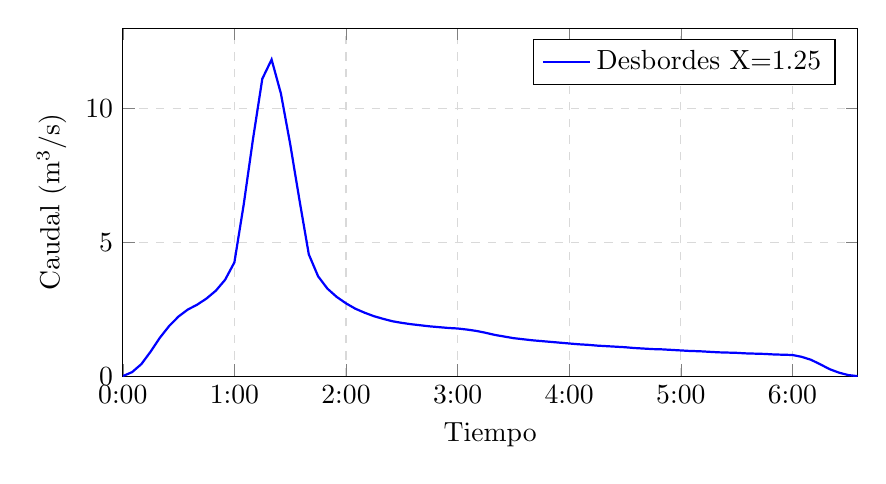
\begin{tikzpicture}
		\begin{axis}[
			width=0.9\textwidth,
			height=6cm,
			xlabel={Tiempo},
			ylabel={Caudal (m$^3$/s)},
			xmin=0,
			xmax=395,
			ymin=0,
			ymax=13,
			grid=major,
			grid style={dashed, gray!30},
			legend pos=north east,
			xtick={0, 60, 120, 180, 240, 300, 360},
			xticklabels={0:00, 1:00, 2:00, 3:00, 4:00, 5:00, 6:00},
			]
		% Desbordes X=1.25
		\addplot [
		blue,
		thick,
		solid,
		] coordinates {
				(0, 0.00) (5, 0.15) (10, 0.45) (15, 0.92) (20, 1.44)
				(25, 1.88) (30, 2.23) (35, 2.49) (40, 2.67) (45, 2.90)
				(50, 3.19) (55, 3.60) (60, 4.25) (65, 6.41) (70, 8.86)
				(75, 11.11) (80, 11.83) (85, 10.56) (90, 8.67) (95, 6.57)
				(100, 4.55) (105, 3.73) (110, 3.27) (115, 2.96) (120, 2.72)
				(125, 2.52) (130, 2.37) (135, 2.24) (140, 2.14) (145, 2.05)
				(150, 1.99) (155, 1.94) (160, 1.90) (165, 1.86) (170, 1.83)
				(175, 1.80) (180, 1.78) (185, 1.74) (190, 1.69) (195, 1.62)
				(200, 1.54) (205, 1.48) (210, 1.42) (215, 1.38) (220, 1.34)
				(225, 1.31) (230, 1.28) (235, 1.25) (240, 1.22) (245, 1.19)
				(250, 1.17) (255, 1.14) (260, 1.12) (265, 1.10) (270, 1.08)
				(275, 1.05) (280, 1.03) (285, 1.01) (290, 1.00) (295, 0.98)
				(300, 0.96) (305, 0.94) (310, 0.93) (315, 0.91) (320, 0.89)
				(325, 0.88) (330, 0.87) (335, 0.85) (340, 0.84) (345, 0.83)
				(350, 0.81) (355, 0.80) (360, 0.79) (365, 0.72) (370, 0.61)
				(375, 0.44) (380, 0.26) (385, 0.13) (390, 0.04) (395, 0.00)
		};
		\addlegendentry{Desbordes X=1.25}

		\end{axis}
	\end{tikzpicture}
	\caption{Hidrograma - Desbordes + GZ $T_r$=25 años ($Q_p$=11.833 m$^3$/s)}
	\label{fig:hydro_desbordes_gz_Tr25_X125}
\end{figure}
}
\end{minipage}
\caption{Hietograma e Hidrograma - Desbordes + GZ $T_r$=25 años X=1.25}
\end{figure}

\subsection{Kirpich + BLOCKS $T_r$=10 años }

% Tabla de parámetros del análisis
\begin{table}[H]
\centering
\small
\begin{tabular}{lr|lr}
\toprule
\multicolumn{2}{c|}{\textbf{Entrada}} & \multicolumn{2}{c}{\textbf{Resultados}} \\
\midrule
Método $T_c$ & Kirpich & Precipitación & 51.1 mm \\
$T_c$ & 12.3 min & Escorrentía & 31.7 mm \\
Tormenta & BLOCKS & $Q_p$ & \textbf{14.047 m$^3$/s} \\
$T_r$ & 10 años & $T_p$ & 40.0 min \\
 &  & Volumen & 19895 m$^3$ \\
\bottomrule
\end{tabular}
\caption{Ficha técnica: Kirpich + BLOCKS $T_r$=10 años }
\end{table}

% Hietograma e Hidrograma
\begin{figure}[H]
\centering
\begin{minipage}{0.48\textwidth}
\centering
\resizebox{\textwidth}{!}{\begin{figure}[H]
	\centering
	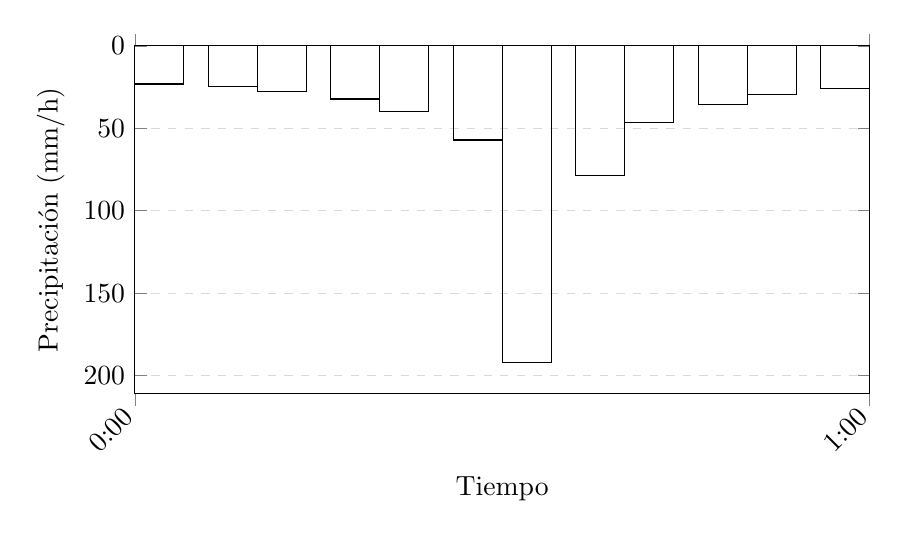
\begin{tikzpicture}
		\begin{axis}[
			width=0.9\textwidth,
			height=6cm,
			xlabel={Tiempo},
			ylabel={Precipitación (mm/h)},
			y dir=reverse,
			ymin=0,
			ymax=211,
			xmin=0,
			xmax=60,
			ybar,
			bar width=4,
			xtick={0, 60},
			xticklabels={0:00, 1:00},
			xticklabel style={rotate=45, anchor=east},
			grid=major,
			grid style={dashed, gray!30},
			]
			\addplot [
			draw=black,
			fill=none
			]
			coordinates {
				(2, 23.16) (8, 24.60) (12, 27.72) (18, 32.28) (22, 40.08)
				(28, 57.12) (32, 192.00) (38, 78.72) (42, 46.56) (48, 35.64)
				(52, 29.76) (58, 25.92)
			};
		\end{axis}
	\end{tikzpicture}
	\caption{Hietograma - BLOCKS $T_r$=10 años (P=51.1 mm)}
	\label{fig:hyeto_kirpich_blocks_Tr10}
\end{figure}
}
\end{minipage}
\hfill
\begin{minipage}{0.48\textwidth}
\centering
\resizebox{\textwidth}{!}{\begin{figure}[H]
	\centering
	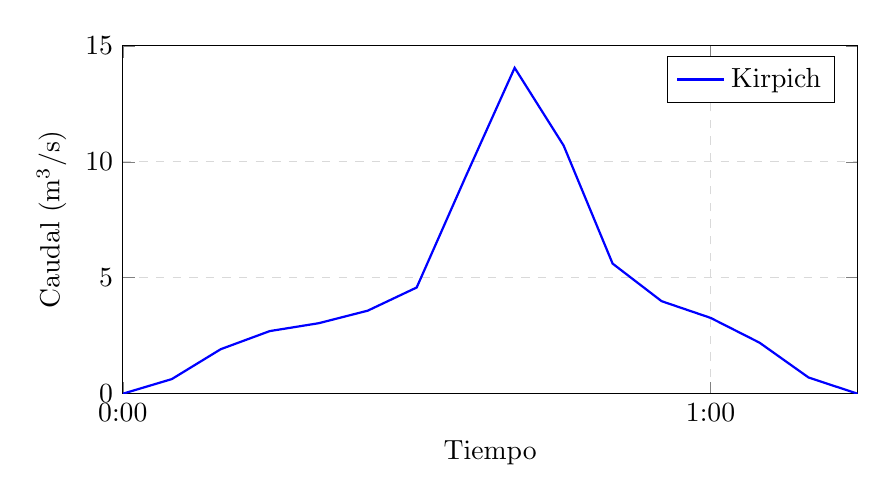
\begin{tikzpicture}
		\begin{axis}[
			width=0.9\textwidth,
			height=6cm,
			xlabel={Tiempo},
			ylabel={Caudal (m$^3$/s)},
			xmin=0,
			xmax=75,
			ymin=0,
			ymax=15,
			grid=major,
			grid style={dashed, gray!30},
			legend pos=north east,
			xtick={0, 60},
			xticklabels={0:00, 1:00},
			]
		% Kirpich
		\addplot [
		blue,
		thick,
		solid,
		] coordinates {
				(0, 0.00) (5, 0.63) (10, 1.92) (15, 2.70) (20, 3.04)
				(25, 3.58) (30, 4.58) (35, 9.36) (40, 14.05) (45, 10.70)
				(50, 5.61) (55, 3.99) (60, 3.27) (65, 2.20) (70, 0.70)
				(75, 0.00)
		};
		\addlegendentry{Kirpich}

		\end{axis}
	\end{tikzpicture}
	\caption{Hidrograma - Kirpich + BLOCKS $T_r$=10 años ($Q_p$=14.047 m$^3$/s)}
	\label{fig:hydro_kirpich_blocks_Tr10}
\end{figure}
}
\end{minipage}
\caption{Hietograma e Hidrograma - Kirpich + BLOCKS $T_r$=10 años }
\end{figure}

\subsection{Kirpich + BLOCKS $T_r$=25 años }

% Tabla de parámetros del análisis
\begin{table}[H]
\centering
\small
\begin{tabular}{lr|lr}
\toprule
\multicolumn{2}{c|}{\textbf{Entrada}} & \multicolumn{2}{c}{\textbf{Resultados}} \\
\midrule
Método $T_c$ & Kirpich & Precipitación & 60.2 mm \\
$T_c$ & 12.3 min & Escorrentía & 37.3 mm \\
Tormenta & BLOCKS & $Q_p$ & \textbf{16.541 m$^3$/s} \\
$T_r$ & 25 años & $T_p$ & 40.0 min \\
 &  & Volumen & 23429 m$^3$ \\
\bottomrule
\end{tabular}
\caption{Ficha técnica: Kirpich + BLOCKS $T_r$=25 años }
\end{table}

% Hietograma e Hidrograma
\begin{figure}[H]
\centering
\begin{minipage}{0.48\textwidth}
\centering
\resizebox{\textwidth}{!}{\input{hietograma_kirpich_blocks_Tr25.tex}}
\end{minipage}
\hfill
\begin{minipage}{0.48\textwidth}
\centering
\resizebox{\textwidth}{!}{\begin{figure}[H]
	\centering
	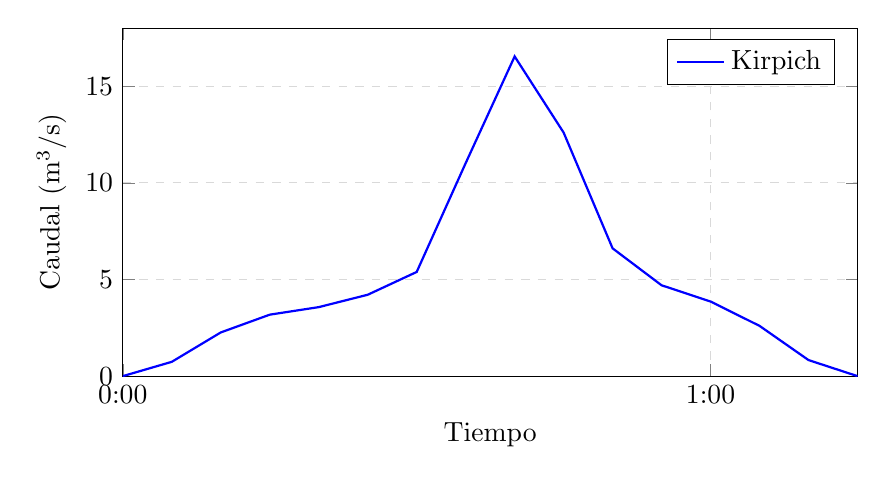
\begin{tikzpicture}
		\begin{axis}[
			width=0.9\textwidth,
			height=6cm,
			xlabel={Tiempo},
			ylabel={Caudal (m$^3$/s)},
			xmin=0,
			xmax=75,
			ymin=0,
			ymax=18,
			grid=major,
			grid style={dashed, gray!30},
			legend pos=north east,
			xtick={0, 60},
			xticklabels={0:00, 1:00},
			]
		% Kirpich
		\addplot [
		blue,
		thick,
		solid,
		] coordinates {
				(0, 0.00) (5, 0.74) (10, 2.26) (15, 3.18) (20, 3.57)
				(25, 4.21) (30, 5.39) (35, 11.02) (40, 16.54) (45, 12.60)
				(50, 6.61) (55, 4.70) (60, 3.86) (65, 2.60) (70, 0.83)
				(75, 0.00)
		};
		\addlegendentry{Kirpich}

		\end{axis}
	\end{tikzpicture}
	\caption{Hidrograma - Kirpich + BLOCKS $T_r$=25 años ($Q_p$=16.541 m$^3$/s)}
	\label{fig:hydro_kirpich_blocks_Tr25}
\end{figure}
}
\end{minipage}
\caption{Hietograma e Hidrograma - Kirpich + BLOCKS $T_r$=25 años }
\end{figure}

\subsection{Desbordes + BLOCKS $T_r$=10 años }

% Tabla de parámetros del análisis
\begin{table}[H]
\centering
\small
\begin{tabular}{lr|lr}
\toprule
\multicolumn{2}{c|}{\textbf{Entrada}} & \multicolumn{2}{c}{\textbf{Resultados}} \\
\midrule
Método $T_c$ & Desbordes & Precipitación & 51.1 mm \\
$T_c$ & 22.6 min & Escorrentía & 31.7 mm \\
Tormenta & BLOCKS & $Q_p$ & \textbf{10.426 m$^3$/s} \\
$T_r$ & 10 años & $T_p$ & 50.0 min \\
 &  & Volumen & 21027 m$^3$ \\
\bottomrule
\end{tabular}
\caption{Ficha técnica: Desbordes + BLOCKS $T_r$=10 años }
\end{table}

% Hietograma e Hidrograma
\begin{figure}[H]
\centering
\begin{minipage}{0.48\textwidth}
\centering
\resizebox{\textwidth}{!}{\input{hietograma_desbordes_blocks_Tr10.tex}}
\end{minipage}
\hfill
\begin{minipage}{0.48\textwidth}
\centering
\resizebox{\textwidth}{!}{\begin{figure}[H]
	\centering
	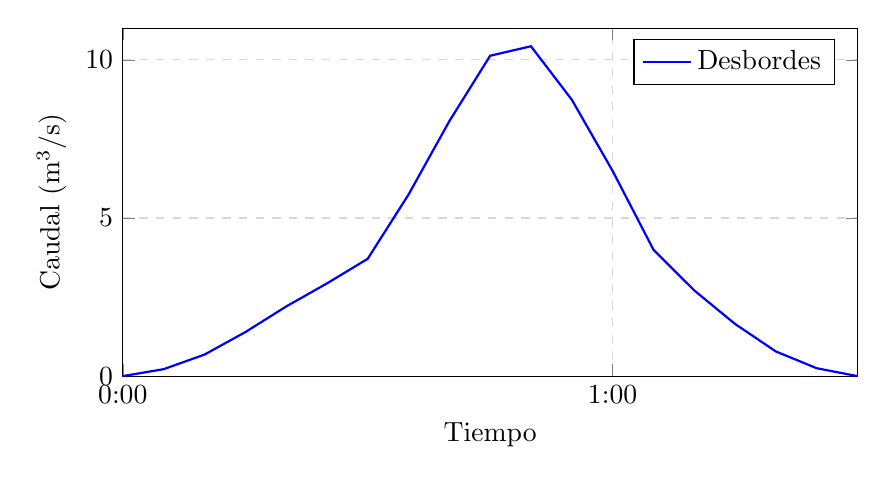
\begin{tikzpicture}
		\begin{axis}[
			width=0.9\textwidth,
			height=6cm,
			xlabel={Tiempo},
			ylabel={Caudal (m$^3$/s)},
			xmin=0,
			xmax=90,
			ymin=0,
			ymax=11,
			grid=major,
			grid style={dashed, gray!30},
			legend pos=north east,
			xtick={0, 60},
			xticklabels={0:00, 1:00},
			]
		% Desbordes
		\addplot [
		blue,
		thick,
		solid,
		] coordinates {
				(0, 0.00) (5, 0.22) (10, 0.68) (15, 1.39) (20, 2.20)
				(25, 2.93) (30, 3.71) (35, 5.74) (40, 8.06) (45, 10.13)
				(50, 10.43) (55, 8.74) (60, 6.49) (65, 4.00) (70, 2.71)
				(75, 1.65) (80, 0.78) (85, 0.25) (90, 0.00)
		};
		\addlegendentry{Desbordes}

		\end{axis}
	\end{tikzpicture}
	\caption{Hidrograma - Desbordes + BLOCKS $T_r$=10 años ($Q_p$=10.426 m$^3$/s)}
	\label{fig:hydro_desbordes_blocks_Tr10}
\end{figure}
}
\end{minipage}
\caption{Hietograma e Hidrograma - Desbordes + BLOCKS $T_r$=10 años }
\end{figure}

\subsection{Desbordes + BLOCKS $T_r$=25 años }

% Tabla de parámetros del análisis
\begin{table}[H]
\centering
\small
\begin{tabular}{lr|lr}
\toprule
\multicolumn{2}{c|}{\textbf{Entrada}} & \multicolumn{2}{c}{\textbf{Resultados}} \\
\midrule
Método $T_c$ & Desbordes & Precipitación & 60.2 mm \\
$T_c$ & 22.6 min & Escorrentía & 37.3 mm \\
Tormenta & BLOCKS & $Q_p$ & \textbf{12.278 m$^3$/s} \\
$T_r$ & 25 años & $T_p$ & 50.0 min \\
 &  & Volumen & 24761 m$^3$ \\
\bottomrule
\end{tabular}
\caption{Ficha técnica: Desbordes + BLOCKS $T_r$=25 años }
\end{table}

% Hietograma e Hidrograma
\begin{figure}[H]
\centering
\begin{minipage}{0.48\textwidth}
\centering
\resizebox{\textwidth}{!}{\begin{figure}[H]
	\centering
	\begin{tikzpicture}
		\begin{axis}[
			width=0.9\textwidth,
			height=6cm,
			xlabel={Tiempo},
			ylabel={Precipitación (mm/h)},
			y dir=reverse,
			ymin=0,
			ymax=249,
			xmin=0,
			xmax=60,
			ybar,
			bar width=4,
			xtick={0, 60},
			xticklabels={0:00, 1:00},
			xticklabel style={rotate=45, anchor=east},
			grid=major,
			grid style={dashed, gray!30},
			]
			\addplot [
			draw=black,
			fill=none
			]
			coordinates {
				(2, 27.36) (8, 28.80) (12, 32.64) (18, 38.04) (22, 47.16)
				(28, 67.20) (32, 226.08) (38, 92.76) (42, 54.84) (48, 42.00)
				(52, 35.04) (58, 30.60)
			};
		\end{axis}
	\end{tikzpicture}
	\caption{Hietograma - BLOCKS $T_r$=25 años (P=60.2 mm)}
	\label{fig:hyeto_desbordes_blocks_Tr25}
\end{figure}
}
\end{minipage}
\hfill
\begin{minipage}{0.48\textwidth}
\centering
\resizebox{\textwidth}{!}{\begin{figure}[H]
	\centering
	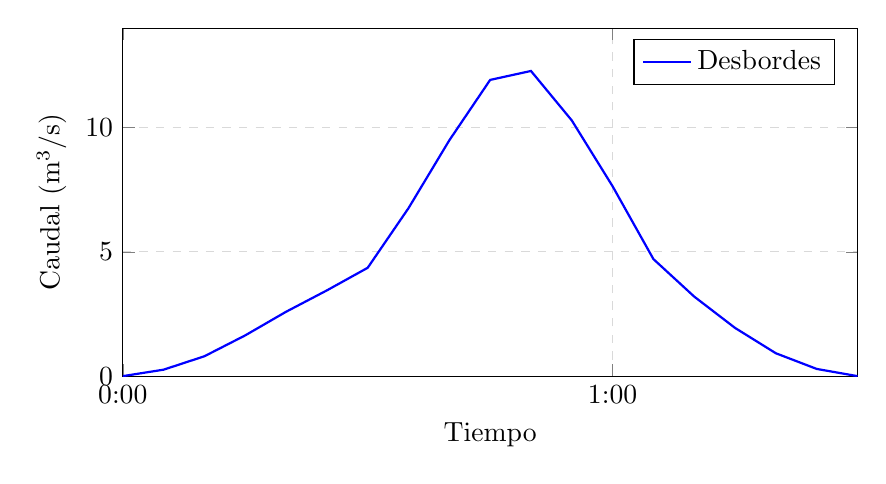
\begin{tikzpicture}
		\begin{axis}[
			width=0.9\textwidth,
			height=6cm,
			xlabel={Tiempo},
			ylabel={Caudal (m$^3$/s)},
			xmin=0,
			xmax=90,
			ymin=0,
			ymax=14,
			grid=major,
			grid style={dashed, gray!30},
			legend pos=north east,
			xtick={0, 60},
			xticklabels={0:00, 1:00},
			]
		% Desbordes
		\addplot [
		blue,
		thick,
		solid,
		] coordinates {
				(0, 0.00) (5, 0.26) (10, 0.80) (15, 1.64) (20, 2.59)
				(25, 3.45) (30, 4.36) (35, 6.76) (40, 9.49) (45, 11.92)
				(50, 12.28) (55, 10.29) (60, 7.64) (65, 4.71) (70, 3.20)
				(75, 1.94) (80, 0.92) (85, 0.29) (90, 0.00)
		};
		\addlegendentry{Desbordes}

		\end{axis}
	\end{tikzpicture}
	\caption{Hidrograma - Desbordes + BLOCKS $T_r$=25 años ($Q_p$=12.278 m$^3$/s)}
	\label{fig:hydro_desbordes_blocks_Tr25}
\end{figure}
}
\end{minipage}
\caption{Hietograma e Hidrograma - Desbordes + BLOCKS $T_r$=25 años }
\end{figure}

\subsection{Kirpich + BLOCKS24 $T_r$=10 años }

% Tabla de parámetros del análisis
\begin{table}[H]
\centering
\small
\begin{tabular}{lr|lr}
\toprule
\multicolumn{2}{c|}{\textbf{Entrada}} & \multicolumn{2}{c}{\textbf{Resultados}} \\
\midrule
Método $T_c$ & Kirpich & Precipitación & 151.8 mm \\
$T_c$ & 12.3 min & Escorrentía & 94.1 mm \\
Tormenta & BLOCKS24 & $Q_p$ & \textbf{10.767 m$^3$/s} \\
$T_r$ & 10 años & $T_p$ & 740.0 min \\
 &  & Volumen & 62853 m$^3$ \\
\bottomrule
\end{tabular}
\caption{Ficha técnica: Kirpich + BLOCKS24 $T_r$=10 años }
\end{table}

% Hietograma e Hidrograma
\begin{figure}[H]
\centering
\begin{minipage}{0.48\textwidth}
\centering
\resizebox{\textwidth}{!}{\begin{figure}[H]
	\centering
	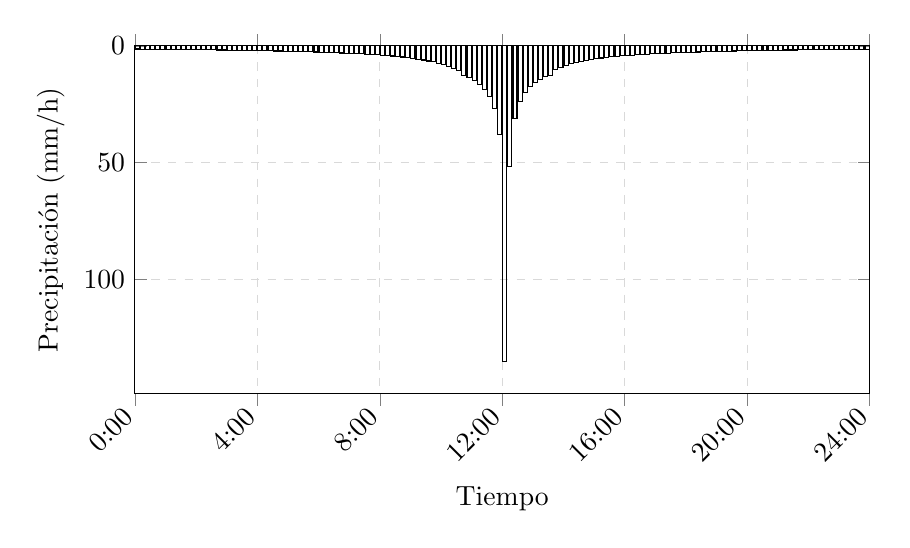
\begin{tikzpicture}
		\begin{axis}[
			width=0.9\textwidth,
			height=6cm,
			xlabel={Tiempo},
			ylabel={Precipitación (mm/h)},
			y dir=reverse,
			ymin=0,
			ymax=149,
			xmin=0,
			xmax=1440,
			ybar,
			bar width=8,
			xtick={0, 240, 480, 720, 960, 1200, 1440},
			xticklabels={0:00, 4:00, 8:00, 12:00, 16:00, 20:00, 24:00},
			xticklabel style={rotate=45, anchor=east},
			grid=major,
			grid style={dashed, gray!30},
			]
			\addplot [
			draw=black,
			fill=none
			]
			coordinates {
				(5, 1.38) (15, 1.44) (25, 1.44) (35, 1.50) (45, 1.50)
				(55, 1.50) (65, 1.56) (75, 1.56) (85, 1.56) (95, 1.62)
				(105, 1.62) (115, 1.68) (125, 1.68) (135, 1.68) (145, 1.74)
				(155, 1.74) (165, 1.80) (175, 1.80) (185, 1.86) (195, 1.86)
				(205, 1.92) (215, 1.98) (225, 1.98) (235, 2.04) (245, 2.10)
				(255, 2.10) (265, 2.16) (275, 2.22) (285, 2.22) (295, 2.28)
				(305, 2.34) (315, 2.40) (325, 2.46) (335, 2.52) (345, 2.58)
				(355, 2.64) (365, 2.70) (375, 2.82) (385, 2.88) (395, 2.94)
				(405, 3.06) (415, 3.12) (425, 3.30) (435, 3.36) (445, 3.48)
				(455, 3.60) (465, 3.72) (475, 3.90) (485, 4.02) (495, 4.26)
				(505, 4.38) (515, 4.68) (525, 4.80) (535, 5.10) (545, 5.40)
				(555, 5.70) (565, 6.06) (575, 6.48) (585, 6.90) (595, 7.50)
				(605, 8.10) (615, 8.82) (625, 9.66) (635, 10.74) (645, 12.78)
				(655, 13.68) (665, 14.88) (675, 16.50) (685, 18.60) (695, 21.72)
				(705, 26.82) (715, 37.86) (725, 135.36) (735, 51.84) (745, 31.02)
				(755, 23.88) (765, 19.98) (775, 17.46) (785, 15.66) (795, 14.34)
				(805, 13.20) (815, 12.66) (825, 10.20) (835, 9.24) (845, 8.46)
				(855, 7.74) (865, 7.20) (875, 6.72) (885, 6.30) (895, 5.88)
				(905, 5.58) (915, 5.22) (925, 5.04) (935, 4.74) (945, 4.50)
				(955, 4.32) (965, 4.14) (975, 3.96) (985, 3.84) (995, 3.66)
				(1005, 3.54) (1015, 3.42) (1025, 3.30) (1035, 3.18) (1045, 3.12)
				(1055, 3.00) (1065, 2.94) (1075, 2.82) (1085, 2.76) (1095, 2.70)
				(1105, 2.64) (1115, 2.52) (1125, 2.52) (1135, 2.40) (1145, 2.40)
				(1155, 2.34) (1165, 2.28) (1175, 2.22) (1185, 2.16) (1195, 2.10)
				(1205, 2.10) (1215, 2.04) (1225, 1.98) (1235, 1.98) (1245, 1.92)
				(1255, 1.92) (1265, 1.86) (1275, 1.80) (1285, 1.80) (1295, 1.80)
				(1305, 1.74) (1315, 1.74) (1325, 1.68) (1335, 1.68) (1345, 1.62)
				(1355, 1.62) (1365, 1.56) (1375, 1.56) (1385, 1.56) (1395, 1.56)
				(1405, 1.50) (1415, 1.50) (1425, 1.44) (1435, 1.44)
			};
		\end{axis}
	\end{tikzpicture}
	\caption{Hietograma - BLOCKS24 $T_r$=10 años (P=151.8 mm)}
	\label{fig:hyeto_kirpich_blocks24_Tr10}
\end{figure}
}
\end{minipage}
\hfill
\begin{minipage}{0.48\textwidth}
\centering
\resizebox{\textwidth}{!}{\begin{figure}[H]
	\centering
	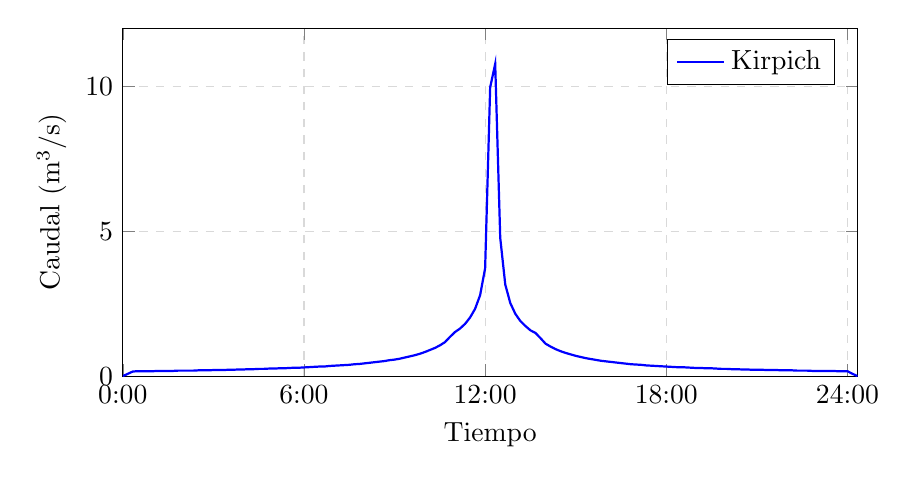
\begin{tikzpicture}
		\begin{axis}[
			width=0.9\textwidth,
			height=6cm,
			xlabel={Tiempo},
			ylabel={Caudal (m$^3$/s)},
			xmin=0,
			xmax=1460,
			ymin=0,
			ymax=12,
			grid=major,
			grid style={dashed, gray!30},
			legend pos=north east,
			xtick={0, 360, 720, 1080, 1440},
			xticklabels={0:00, 6:00, 12:00, 18:00, 24:00},
			]
		% Kirpich
		\addplot [
		blue,
		thick,
		solid,
		] coordinates {
				(0, 0.00) (10, 0.08) (20, 0.16) (30, 0.17) (40, 0.17)
				(50, 0.17) (60, 0.17) (70, 0.18) (80, 0.18) (90, 0.18)
				(100, 0.18) (110, 0.19) (120, 0.19) (130, 0.19) (140, 0.19)
				(150, 0.20) (160, 0.20) (170, 0.20) (180, 0.21) (190, 0.21)
				(200, 0.21) (210, 0.22) (220, 0.22) (230, 0.23) (240, 0.23)
				(250, 0.24) (260, 0.24) (270, 0.25) (280, 0.25) (290, 0.26)
				(300, 0.26) (310, 0.27) (320, 0.27) (330, 0.28) (340, 0.29)
				(350, 0.29) (360, 0.30) (370, 0.31) (380, 0.32) (390, 0.33)
				(400, 0.33) (410, 0.35) (420, 0.36) (430, 0.37) (440, 0.38)
				(450, 0.39) (460, 0.41) (470, 0.42) (480, 0.44) (490, 0.46)
				(500, 0.48) (510, 0.50) (520, 0.52) (530, 0.55) (540, 0.57)
				(550, 0.60) (560, 0.64) (570, 0.68) (580, 0.72) (590, 0.77)
				(600, 0.83) (610, 0.90) (620, 0.97) (630, 1.06) (640, 1.17)
				(650, 1.35) (660, 1.52) (670, 1.64) (680, 1.80) (690, 2.02)
				(700, 2.32) (710, 2.79) (720, 3.72) (730, 9.96) (740, 10.77)
				(750, 4.77) (760, 3.16) (770, 2.52) (780, 2.15) (790, 1.90)
				(800, 1.73) (810, 1.58) (820, 1.49) (830, 1.31) (840, 1.12)
				(850, 1.02) (860, 0.93) (870, 0.86) (880, 0.80) (890, 0.75)
				(900, 0.70) (910, 0.66) (920, 0.62) (930, 0.59) (940, 0.56)
				(950, 0.53) (960, 0.51) (970, 0.49) (980, 0.47) (990, 0.45)
				(1000, 0.43) (1010, 0.41) (1020, 0.40) (1030, 0.39) (1040, 0.37)
				(1050, 0.36) (1060, 0.35) (1070, 0.34) (1080, 0.33) (1090, 0.32)
				(1100, 0.31) (1110, 0.31) (1120, 0.30) (1130, 0.29) (1140, 0.28)
				(1150, 0.28) (1160, 0.27) (1170, 0.27) (1180, 0.26) (1190, 0.25)
				(1200, 0.25) (1210, 0.24) (1220, 0.24) (1230, 0.23) (1240, 0.23)
				(1250, 0.22) (1260, 0.22) (1270, 0.22) (1280, 0.21) (1290, 0.21)
				(1300, 0.21) (1310, 0.20) (1320, 0.20) (1330, 0.20) (1340, 0.19)
				(1350, 0.19) (1360, 0.19) (1370, 0.18) (1380, 0.18) (1390, 0.18)
				(1400, 0.18) (1410, 0.18) (1420, 0.17) (1430, 0.17) (1440, 0.17)
				(1450, 0.08) (1460, 0.00)
		};
		\addlegendentry{Kirpich}

		\end{axis}
	\end{tikzpicture}
	\caption{Hidrograma - Kirpich + BLOCKS24 $T_r$=10 años ($Q_p$=10.767 m$^3$/s)}
	\label{fig:hydro_kirpich_blocks24_Tr10}
\end{figure}
}
\end{minipage}
\caption{Hietograma e Hidrograma - Kirpich + BLOCKS24 $T_r$=10 años }
\end{figure}

\subsection{Kirpich + BLOCKS24 $T_r$=25 años }

% Tabla de parámetros del análisis
\begin{table}[H]
\centering
\small
\begin{tabular}{lr|lr}
\toprule
\multicolumn{2}{c|}{\textbf{Entrada}} & \multicolumn{2}{c}{\textbf{Resultados}} \\
\midrule
Método $T_c$ & Kirpich & Precipitación & 178.7 mm \\
$T_c$ & 12.3 min & Escorrentía & 110.8 mm \\
Tormenta & BLOCKS24 & $Q_p$ & \textbf{12.679 m$^3$/s} \\
$T_r$ & 25 años & $T_p$ & 740.0 min \\
 &  & Volumen & 74013 m$^3$ \\
\bottomrule
\end{tabular}
\caption{Ficha técnica: Kirpich + BLOCKS24 $T_r$=25 años }
\end{table}

% Hietograma e Hidrograma
\begin{figure}[H]
\centering
\begin{minipage}{0.48\textwidth}
\centering
\resizebox{\textwidth}{!}{\input{hietograma_kirpich_blocks24_Tr25.tex}}
\end{minipage}
\hfill
\begin{minipage}{0.48\textwidth}
\centering
\resizebox{\textwidth}{!}{\begin{figure}[H]
	\centering
	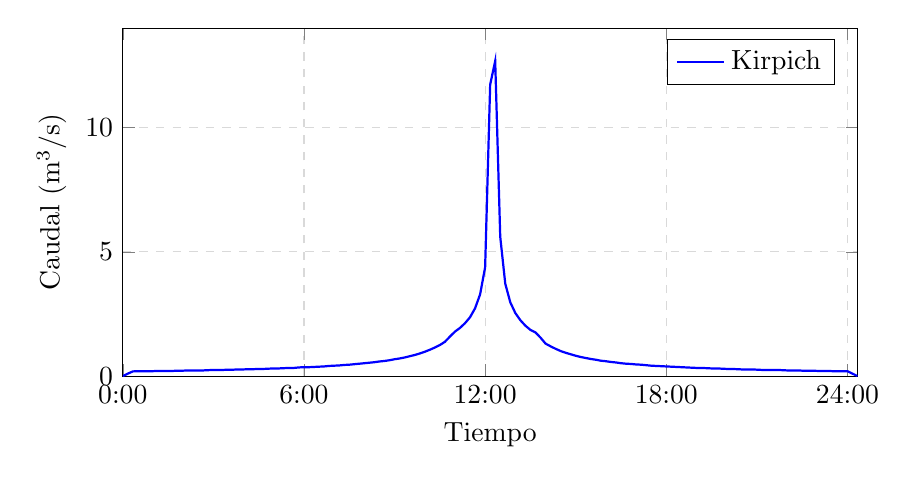
\begin{tikzpicture}
		\begin{axis}[
			width=0.9\textwidth,
			height=6cm,
			xlabel={Tiempo},
			ylabel={Caudal (m$^3$/s)},
			xmin=0,
			xmax=1460,
			ymin=0,
			ymax=14,
			grid=major,
			grid style={dashed, gray!30},
			legend pos=north east,
			xtick={0, 360, 720, 1080, 1440},
			xticklabels={0:00, 6:00, 12:00, 18:00, 24:00},
			]
		% Kirpich
		\addplot [
		blue,
		thick,
		solid,
		] coordinates {
				(0, 0.00) (10, 0.10) (20, 0.19) (30, 0.20) (40, 0.20)
				(50, 0.20) (60, 0.20) (70, 0.21) (80, 0.21) (90, 0.21)
				(100, 0.21) (110, 0.22) (120, 0.22) (130, 0.23) (140, 0.23)
				(150, 0.23) (160, 0.23) (170, 0.24) (180, 0.25) (190, 0.25)
				(200, 0.25) (210, 0.26) (220, 0.26) (230, 0.27) (240, 0.27)
				(250, 0.28) (260, 0.28) (270, 0.29) (280, 0.29) (290, 0.30)
				(300, 0.31) (310, 0.31) (320, 0.32) (330, 0.33) (340, 0.33)
				(350, 0.35) (360, 0.36) (370, 0.36) (380, 0.37) (390, 0.38)
				(400, 0.39) (410, 0.41) (420, 0.42) (430, 0.43) (440, 0.45)
				(450, 0.46) (460, 0.48) (470, 0.50) (480, 0.52) (490, 0.54)
				(500, 0.56) (510, 0.59) (520, 0.61) (530, 0.64) (540, 0.68)
				(550, 0.71) (560, 0.75) (570, 0.80) (580, 0.85) (590, 0.91)
				(600, 0.98) (610, 1.06) (620, 1.15) (630, 1.25) (640, 1.38)
				(650, 1.59) (660, 1.79) (670, 1.94) (680, 2.13) (690, 2.37)
				(700, 2.73) (710, 3.29) (720, 4.38) (730, 11.73) (740, 12.68)
				(750, 5.61) (760, 3.72) (770, 2.97) (780, 2.54) (790, 2.25)
				(800, 2.03) (810, 1.86) (820, 1.76) (830, 1.55) (840, 1.31)
				(850, 1.20) (860, 1.10) (870, 1.01) (880, 0.94) (890, 0.88)
				(900, 0.82) (910, 0.77) (920, 0.73) (930, 0.69) (940, 0.66)
				(950, 0.62) (960, 0.60) (970, 0.57) (980, 0.55) (990, 0.52)
				(1000, 0.50) (1010, 0.49) (1020, 0.47) (1030, 0.46) (1040, 0.44)
				(1050, 0.42) (1060, 0.41) (1070, 0.40) (1080, 0.39) (1090, 0.38)
				(1100, 0.37) (1110, 0.36) (1120, 0.35) (1130, 0.34) (1140, 0.33)
				(1150, 0.33) (1160, 0.32) (1170, 0.31) (1180, 0.31) (1190, 0.30)
				(1200, 0.29) (1210, 0.29) (1220, 0.28) (1230, 0.27) (1240, 0.27)
				(1250, 0.27) (1260, 0.26) (1270, 0.25) (1280, 0.25) (1290, 0.25)
				(1300, 0.25) (1310, 0.24) (1320, 0.23) (1330, 0.23) (1340, 0.23)
				(1350, 0.22) (1360, 0.22) (1370, 0.22) (1380, 0.21) (1390, 0.21)
				(1400, 0.21) (1410, 0.20) (1420, 0.20) (1430, 0.20) (1440, 0.20)
				(1450, 0.10) (1460, 0.00)
		};
		\addlegendentry{Kirpich}

		\end{axis}
	\end{tikzpicture}
	\caption{Hidrograma - Kirpich + BLOCKS24 $T_r$=25 años ($Q_p$=12.679 m$^3$/s)}
	\label{fig:hydro_kirpich_blocks24_Tr25}
\end{figure}
}
\end{minipage}
\caption{Hietograma e Hidrograma - Kirpich + BLOCKS24 $T_r$=25 años }
\end{figure}

\subsection{Desbordes + BLOCKS24 $T_r$=10 años }

% Tabla de parámetros del análisis
\begin{table}[H]
\centering
\small
\begin{tabular}{lr|lr}
\toprule
\multicolumn{2}{c|}{\textbf{Entrada}} & \multicolumn{2}{c}{\textbf{Resultados}} \\
\midrule
Método $T_c$ & Desbordes & Precipitación & 151.8 mm \\
$T_c$ & 22.6 min & Escorrentía & 94.1 mm \\
Tormenta & BLOCKS24 & $Q_p$ & \textbf{10.389 m$^3$/s} \\
$T_r$ & 10 años & $T_p$ & 740.0 min \\
 &  & Volumen & 63000 m$^3$ \\
\bottomrule
\end{tabular}
\caption{Ficha técnica: Desbordes + BLOCKS24 $T_r$=10 años }
\end{table}

% Hietograma e Hidrograma
\begin{figure}[H]
\centering
\begin{minipage}{0.48\textwidth}
\centering
\resizebox{\textwidth}{!}{\input{hietograma_desbordes_blocks24_Tr10.tex}}
\end{minipage}
\hfill
\begin{minipage}{0.48\textwidth}
\centering
\resizebox{\textwidth}{!}{\begin{figure}[H]
	\centering
	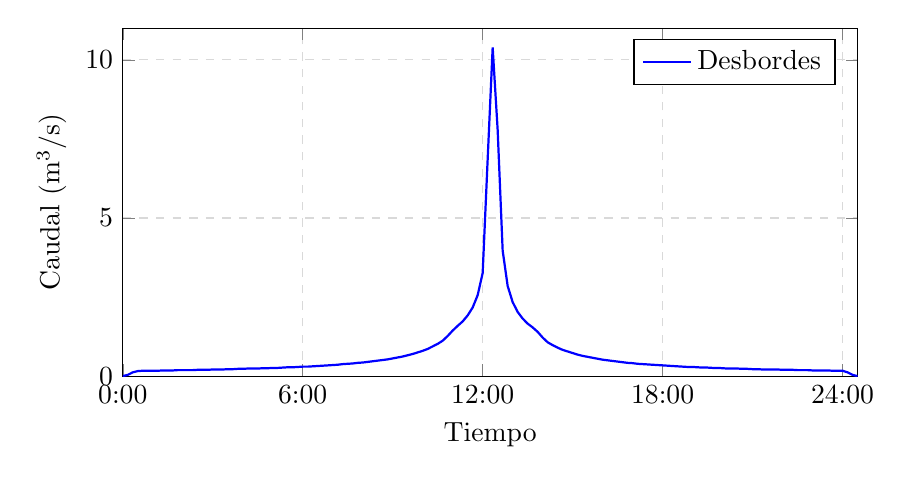
\begin{tikzpicture}
		\begin{axis}[
			width=0.9\textwidth,
			height=6cm,
			xlabel={Tiempo},
			ylabel={Caudal (m$^3$/s)},
			xmin=0,
			xmax=1470,
			ymin=0,
			ymax=11,
			grid=major,
			grid style={dashed, gray!30},
			legend pos=north east,
			xtick={0, 360, 720, 1080, 1440},
			xticklabels={0:00, 6:00, 12:00, 18:00, 24:00},
			]
		% Desbordes
		\addplot [
		blue,
		thick,
		solid,
		] coordinates {
				(0, 0.00) (10, 0.04) (20, 0.12) (30, 0.16) (40, 0.17)
				(50, 0.17) (60, 0.17) (70, 0.17) (80, 0.18) (90, 0.18)
				(100, 0.18) (110, 0.19) (120, 0.19) (130, 0.19) (140, 0.19)
				(150, 0.20) (160, 0.20) (170, 0.20) (180, 0.21) (190, 0.21)
				(200, 0.21) (210, 0.22) (220, 0.22) (230, 0.23) (240, 0.23)
				(250, 0.24) (260, 0.24) (270, 0.24) (280, 0.25) (290, 0.25)
				(300, 0.26) (310, 0.26) (320, 0.27) (330, 0.28) (340, 0.28)
				(350, 0.29) (360, 0.30) (370, 0.30) (380, 0.31) (390, 0.32)
				(400, 0.33) (410, 0.34) (420, 0.35) (430, 0.36) (440, 0.38)
				(450, 0.39) (460, 0.40) (470, 0.42) (480, 0.43) (490, 0.45)
				(500, 0.47) (510, 0.49) (520, 0.51) (530, 0.53) (540, 0.56)
				(550, 0.59) (560, 0.62) (570, 0.66) (580, 0.70) (590, 0.75)
				(600, 0.80) (610, 0.86) (620, 0.94) (630, 1.02) (640, 1.12)
				(650, 1.27) (660, 1.44) (670, 1.59) (680, 1.73) (690, 1.92)
				(700, 2.17) (710, 2.56) (720, 3.26) (730, 6.86) (740, 10.39)
				(750, 7.78) (760, 3.97) (770, 2.85) (780, 2.34) (790, 2.03)
				(800, 1.82) (810, 1.66) (820, 1.54) (830, 1.40) (840, 1.22)
				(850, 1.07) (860, 0.98) (870, 0.90) (880, 0.83) (890, 0.78)
				(900, 0.73) (910, 0.68) (920, 0.64) (930, 0.61) (940, 0.58)
				(950, 0.55) (960, 0.52) (970, 0.50) (980, 0.48) (990, 0.46)
				(1000, 0.44) (1010, 0.42) (1020, 0.41) (1030, 0.39) (1040, 0.38)
				(1050, 0.37) (1060, 0.36) (1070, 0.35) (1080, 0.34) (1090, 0.33)
				(1100, 0.32) (1110, 0.31) (1120, 0.30) (1130, 0.29) (1140, 0.29)
				(1150, 0.28) (1160, 0.27) (1170, 0.27) (1180, 0.26) (1190, 0.26)
				(1200, 0.25) (1210, 0.24) (1220, 0.24) (1230, 0.24) (1240, 0.23)
				(1250, 0.23) (1260, 0.22) (1270, 0.22) (1280, 0.21) (1290, 0.21)
				(1300, 0.21) (1310, 0.21) (1320, 0.20) (1330, 0.20) (1340, 0.20)
				(1350, 0.19) (1360, 0.19) (1370, 0.19) (1380, 0.18) (1390, 0.18)
				(1400, 0.18) (1410, 0.18) (1420, 0.17) (1430, 0.17) (1440, 0.17)
				(1450, 0.12) (1460, 0.04) (1470, 0.00)
		};
		\addlegendentry{Desbordes}

		\end{axis}
	\end{tikzpicture}
	\caption{Hidrograma - Desbordes + BLOCKS24 $T_r$=10 años ($Q_p$=10.389 m$^3$/s)}
	\label{fig:hydro_desbordes_blocks24_Tr10}
\end{figure}
}
\end{minipage}
\caption{Hietograma e Hidrograma - Desbordes + BLOCKS24 $T_r$=10 años }
\end{figure}

\subsection{Desbordes + BLOCKS24 $T_r$=25 años }

% Tabla de parámetros del análisis
\begin{table}[H]
\centering
\small
\begin{tabular}{lr|lr}
\toprule
\multicolumn{2}{c|}{\textbf{Entrada}} & \multicolumn{2}{c}{\textbf{Resultados}} \\
\midrule
Método $T_c$ & Desbordes & Precipitación & 178.7 mm \\
$T_c$ & 22.6 min & Escorrentía & 110.8 mm \\
Tormenta & BLOCKS24 & $Q_p$ & \textbf{12.234 m$^3$/s} \\
$T_r$ & 25 años & $T_p$ & 740.0 min \\
 &  & Volumen & 74187 m$^3$ \\
\bottomrule
\end{tabular}
\caption{Ficha técnica: Desbordes + BLOCKS24 $T_r$=25 años }
\end{table}

% Hietograma e Hidrograma
\begin{figure}[H]
\centering
\begin{minipage}{0.48\textwidth}
\centering
\resizebox{\textwidth}{!}{\begin{figure}[H]
	\centering
	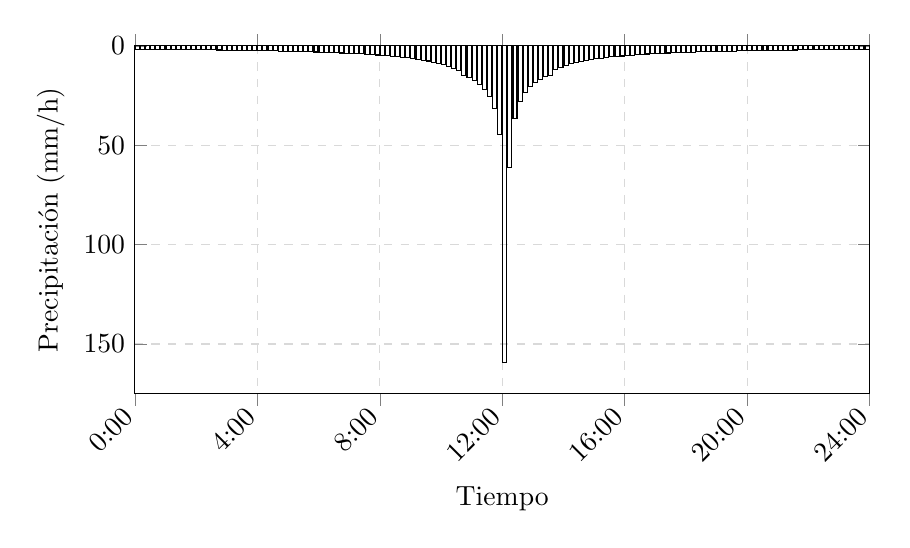
\begin{tikzpicture}
		\begin{axis}[
			width=0.9\textwidth,
			height=6cm,
			xlabel={Tiempo},
			ylabel={Precipitación (mm/h)},
			y dir=reverse,
			ymin=0,
			ymax=175,
			xmin=0,
			xmax=1440,
			ybar,
			bar width=8,
			xtick={0, 240, 480, 720, 960, 1200, 1440},
			xticklabels={0:00, 4:00, 8:00, 12:00, 16:00, 20:00, 24:00},
			xticklabel style={rotate=45, anchor=east},
			grid=major,
			grid style={dashed, gray!30},
			]
			\addplot [
			draw=black,
			fill=none
			]
			coordinates {
				(5, 1.68) (15, 1.68) (25, 1.74) (35, 1.74) (45, 1.74)
				(55, 1.80) (65, 1.80) (75, 1.86) (85, 1.86) (95, 1.86)
				(105, 1.92) (115, 1.98) (125, 1.98) (135, 1.98) (145, 2.04)
				(155, 2.04) (165, 2.10) (175, 2.16) (185, 2.16) (195, 2.22)
				(205, 2.28) (215, 2.28) (225, 2.34) (235, 2.40) (245, 2.46)
				(255, 2.46) (265, 2.52) (275, 2.58) (285, 2.64) (295, 2.70)
				(305, 2.76) (315, 2.82) (325, 2.88) (335, 2.94) (345, 3.06)
				(355, 3.12) (365, 3.18) (375, 3.30) (385, 3.36) (395, 3.48)
				(405, 3.60) (415, 3.72) (425, 3.84) (435, 3.90) (445, 4.08)
				(455, 4.26) (465, 4.44) (475, 4.62) (485, 4.74) (495, 4.98)
				(505, 5.22) (515, 5.46) (525, 5.70) (535, 6.06) (545, 6.36)
				(555, 6.72) (565, 7.20) (575, 7.62) (585, 8.22) (595, 8.82)
				(605, 9.54) (615, 10.38) (625, 11.40) (635, 12.60) (645, 15.00)
				(655, 16.14) (665, 17.58) (675, 19.38) (685, 21.90) (695, 25.56)
				(705, 31.62) (715, 44.58) (725, 159.42) (735, 61.02) (745, 36.54)
				(755, 28.08) (765, 23.52) (775, 20.58) (785, 18.48) (795, 16.80)
				(805, 15.60) (815, 14.94) (825, 12.00) (835, 10.86) (845, 9.96)
				(855, 9.12) (865, 8.46) (875, 7.86) (885, 7.38) (895, 6.90)
				(905, 6.54) (915, 6.18) (925, 5.88) (935, 5.58) (945, 5.28)
				(955, 5.10) (965, 4.86) (975, 4.68) (985, 4.44) (995, 4.32)
				(1005, 4.14) (1015, 4.08) (1025, 3.90) (1035, 3.78) (1045, 3.60)
				(1055, 3.54) (1065, 3.48) (1075, 3.36) (1085, 3.24) (1095, 3.18)
				(1105, 3.06) (1115, 3.00) (1125, 2.94) (1135, 2.88) (1145, 2.82)
				(1155, 2.70) (1165, 2.70) (1175, 2.64) (1185, 2.58) (1195, 2.52)
				(1205, 2.46) (1215, 2.40) (1225, 2.34) (1235, 2.34) (1245, 2.28)
				(1255, 2.22) (1265, 2.16) (1275, 2.16) (1285, 2.16) (1295, 2.10)
				(1305, 2.04) (1315, 2.04) (1325, 1.98) (1335, 1.98) (1345, 1.92)
				(1355, 1.92) (1365, 1.86) (1375, 1.86) (1385, 1.80) (1395, 1.80)
				(1405, 1.74) (1415, 1.74) (1425, 1.74) (1435, 1.68)
			};
		\end{axis}
	\end{tikzpicture}
	\caption{Hietograma - BLOCKS24 $T_r$=25 años (P=178.7 mm)}
	\label{fig:hyeto_desbordes_blocks24_Tr25}
\end{figure}
}
\end{minipage}
\hfill
\begin{minipage}{0.48\textwidth}
\centering
\resizebox{\textwidth}{!}{\begin{figure}[H]
	\centering
	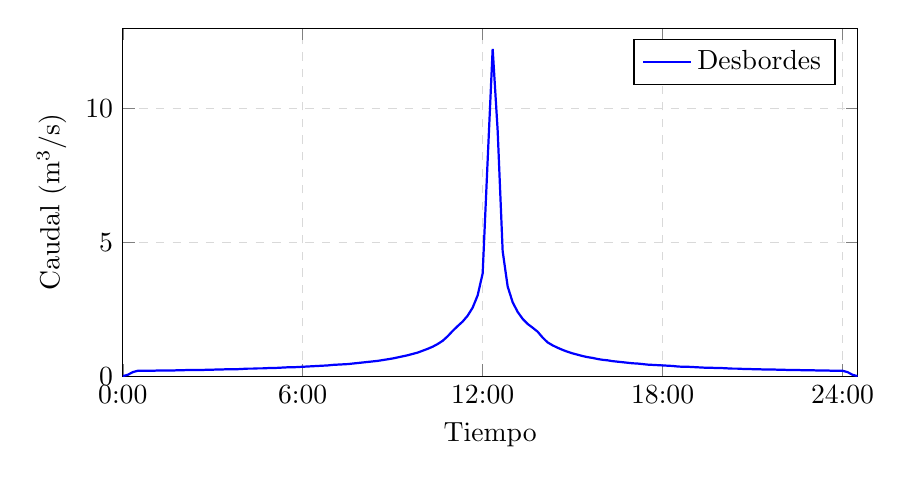
\begin{tikzpicture}
		\begin{axis}[
			width=0.9\textwidth,
			height=6cm,
			xlabel={Tiempo},
			ylabel={Caudal (m$^3$/s)},
			xmin=0,
			xmax=1470,
			ymin=0,
			ymax=13,
			grid=major,
			grid style={dashed, gray!30},
			legend pos=north east,
			xtick={0, 360, 720, 1080, 1440},
			xticklabels={0:00, 6:00, 12:00, 18:00, 24:00},
			]
		% Desbordes
		\addplot [
		blue,
		thick,
		solid,
		] coordinates {
				(0, 0.00) (10, 0.05) (20, 0.15) (30, 0.20) (40, 0.20)
				(50, 0.20) (60, 0.20) (70, 0.21) (80, 0.21) (90, 0.21)
				(100, 0.21) (110, 0.22) (120, 0.22) (130, 0.23) (140, 0.23)
				(150, 0.23) (160, 0.23) (170, 0.24) (180, 0.24) (190, 0.25)
				(200, 0.25) (210, 0.26) (220, 0.26) (230, 0.26) (240, 0.27)
				(250, 0.28) (260, 0.28) (270, 0.29) (280, 0.29) (290, 0.30)
				(300, 0.30) (310, 0.31) (320, 0.32) (330, 0.33) (340, 0.33)
				(350, 0.34) (360, 0.35) (370, 0.36) (380, 0.37) (390, 0.38)
				(400, 0.39) (410, 0.40) (420, 0.42) (430, 0.43) (440, 0.44)
				(450, 0.45) (460, 0.47) (470, 0.49) (480, 0.51) (490, 0.53)
				(500, 0.55) (510, 0.57) (520, 0.60) (530, 0.63) (540, 0.66)
				(550, 0.70) (560, 0.74) (570, 0.78) (580, 0.83) (590, 0.88)
				(600, 0.95) (610, 1.02) (620, 1.10) (630, 1.20) (640, 1.32)
				(650, 1.49) (660, 1.69) (670, 1.87) (680, 2.04) (690, 2.26)
				(700, 2.56) (710, 3.02) (720, 3.84) (730, 8.08) (740, 12.23)
				(750, 9.17) (760, 4.67) (770, 3.35) (780, 2.76) (790, 2.40)
				(800, 2.14) (810, 1.95) (820, 1.81) (830, 1.66) (840, 1.44)
				(850, 1.26) (860, 1.15) (870, 1.06) (880, 0.98) (890, 0.91)
				(900, 0.85) (910, 0.80) (920, 0.75) (930, 0.71) (940, 0.68)
				(950, 0.64) (960, 0.61) (970, 0.59) (980, 0.56) (990, 0.54)
				(1000, 0.52) (1010, 0.50) (1020, 0.48) (1030, 0.47) (1040, 0.45)
				(1050, 0.43) (1060, 0.42) (1070, 0.41) (1080, 0.40) (1090, 0.39)
				(1100, 0.38) (1110, 0.36) (1120, 0.35) (1130, 0.35) (1140, 0.34)
				(1150, 0.33) (1160, 0.32) (1170, 0.31) (1180, 0.31) (1190, 0.30)
				(1200, 0.30) (1210, 0.29) (1220, 0.28) (1230, 0.28) (1240, 0.27)
				(1250, 0.27) (1260, 0.26) (1270, 0.26) (1280, 0.25) (1290, 0.25)
				(1300, 0.25) (1310, 0.24) (1320, 0.24) (1330, 0.23) (1340, 0.23)
				(1350, 0.23) (1360, 0.22) (1370, 0.22) (1380, 0.22) (1390, 0.21)
				(1400, 0.21) (1410, 0.21) (1420, 0.20) (1430, 0.20) (1440, 0.20)
				(1450, 0.15) (1460, 0.05) (1470, 0.00)
		};
		\addlegendentry{Desbordes}

		\end{axis}
	\end{tikzpicture}
	\caption{Hidrograma - Desbordes + BLOCKS24 $T_r$=25 años ($Q_p$=12.234 m$^3$/s)}
	\label{fig:hydro_desbordes_blocks24_Tr25}
\end{figure}
}
\end{minipage}
\caption{Hietograma e Hidrograma - Desbordes + BLOCKS24 $T_r$=25 años }
\end{figure}

